% QSFD Minor Project Report (university format). pdfLaTeX. Build: pdflatex x2 (bibliography is pre-generated).
\documentclass[12pt,a4paper]{report}
\usepackage[utf8]{inputenc}
\usepackage[T1]{fontenc}
\usepackage{ebgaramond}% Garamond, used for captions only
\usepackage{mathptmx}% Times New Roman-compatible text and math (loaded last: sets the main font)
\usepackage[a4paper,top=1in,bottom=1.15in,left=1.5in,right=0.6in,headheight=30pt]{geometry}
\usepackage{amsmath,amssymb}
\usepackage{graphicx}
\usepackage{booktabs,longtable,array,tabularx}
\usepackage{url}
\usepackage{setspace}
\usepackage{enumitem}
\usepackage{fancyhdr}
\usepackage[explicit]{titlesec}
\usepackage{caption}
\usepackage[hidelinks]{hyperref}
\graphicspath{{../common/figures/}{./}}
\setkeys{Gin}{height=0.4\textheight,keepaspectratio=true}
\emergencystretch=3em
\newcommand{\figw}{0.9\textwidth}
\newcommand{\placeholder}[1]{\textbf{[#1 -- to be completed]}}
% AUTO-GENERATED by scripts/final/build_latex_assets.py from results/final/final_results.json -- do not edit
\newcommand{\BbMAE}{0.0028}
\newcommand{\BbMaxDiff}{0.0065}
\newcommand{\BbRMSE}{0.0036}
\newcommand{\BbciProtoHClean}{[0.0000, 0.0000]}
\newcommand{\BbciProtoHEve}{[0.2448, 0.2558]}
\newcommand{\BbciProtoHEveNoise}{[0.2557, 0.2661]}
\newcommand{\BbciProtoHFivePct}{[0.0470, 0.0521]}
\newcommand{\BbciProtoHOnePct}{[0.0090, 0.0118]}
\newcommand{\BbciProtoHTenPct}{[0.0965, 0.1033]}
\newcommand{\BbciProtoKClean}{[0.0000, 0.0000]}
\newcommand{\BbciProtoKEve}{[0.2479, 0.2537]}
\newcommand{\BbciProtoKEveNoise}{[0.2578, 0.2635]}
\newcommand{\BbciProtoKFivePct}{[0.0477, 0.0504]}
\newcommand{\BbciProtoKOnePct}{[0.0091, 0.0103]}
\newcommand{\BbciProtoKTenPct}{[0.0960, 0.0999]}
\newcommand{\BbciQiskClean}{[0.0000, 0.0000]}
\newcommand{\BbciQiskEve}{[0.2360, 0.2515]}
\newcommand{\BbciQiskEveNoise}{[0.2576, 0.2722]}
\newcommand{\BbciQiskFivePct}{[0.0458, 0.0538]}
\newcommand{\BbciQiskOnePct}{[0.0059, 0.0104]}
\newcommand{\BbciQiskTenPct}{[0.0896, 0.1023]}
\newcommand{\BbqProtoHClean}{0.0000}
\newcommand{\BbqProtoHEve}{0.2503}
\newcommand{\BbqProtoHEveNoise}{0.2609}
\newcommand{\BbqProtoHFivePct}{0.0496}
\newcommand{\BbqProtoHOnePct}{0.0104}
\newcommand{\BbqProtoHTenPct}{0.0999}
\newcommand{\BbqProtoKClean}{0.0000}
\newcommand{\BbqProtoKEve}{0.2508}
\newcommand{\BbqProtoKEveNoise}{0.2606}
\newcommand{\BbqProtoKFivePct}{0.0490}
\newcommand{\BbqProtoKOnePct}{0.0097}
\newcommand{\BbqProtoKTenPct}{0.0979}
\newcommand{\BbqQiskClean}{0.0000}
\newcommand{\BbqQiskEve}{0.2438}
\newcommand{\BbqQiskEveNoise}{0.2649}
\newcommand{\BbqQiskFivePct}{0.0498}
\newcommand{\BbqQiskOnePct}{0.0082}
\newcommand{\BbqQiskTenPct}{0.0960}
\newcommand{\CapCIhi}{0.0173}
\newcommand{\CapCIlo}{-0.0035}
\newcommand{\CapXgb}{0.9613}
\newcommand{\CapXgbControl}{0.9671}
\newcommand{\CapXgbGlobal}{0.9632}
\newcommand{\CapXgbLocal}{0.9665}
\newcommand{\ClsIfPr}{0.0397}
\newcommand{\ClsIfRoc}{0.9492}
\newcommand{\ClsLrPr}{0.7328}
\newcommand{\ClsLrRoc}{0.9839}
\newcommand{\ClsRfPr}{0.8191}
\newcommand{\ClsRfRoc}{0.9692}
\newcommand{\ClsXgbPr}{0.8007}
\newcommand{\ClsXgbRoc}{0.9772}
\newcommand{\EEABytes}{475}
\newcommand{\EEAExpansion}{1.5}
\newcommand{\EEAMedian}{0.30}
\newcommand{\EEBTwoBytes}{9284}
\newcommand{\EEBTwoExpansion}{29.8}
\newcommand{\EEBTwoMedian}{3631.69}
\newcommand{\EEBBytes}{4737}
\newcommand{\EEBExpansion}{15.2}
\newcommand{\EEBMedian}{72.83}
\newcommand{\EECTwoBytes}{9284}
\newcommand{\EECTwoExpansion}{29.8}
\newcommand{\EECTwoMedian}{1252.82}
\newcommand{\EECBytes}{4737}
\newcommand{\EECExpansion}{15.2}
\newcommand{\EECMedian}{10.15}
\newcommand{\EEDBytes}{4873}
\newcommand{\EEDExpansion}{15.6}
\newcommand{\EEDMedian}{10.53}
\newcommand{\FezCltDepth}{45}
\newcommand{\FezCltMAD}{0.229}
\newcommand{\FezCltPearson}{0.43}
\newcommand{\FezLinearDepth}{47}
\newcommand{\FezLinearMAD}{0.417}
\newcommand{\FezLinearPearson}{0.16}
\newcommand{\HwAsymCells}{11/15}
\newcommand{\HwAsymOneBest}{0.0099}
\newcommand{\HwAsymOneTypical}{0.0113}
\newcommand{\HwAsymOneWorse}{0.0339}
\newcommand{\HwAsymZeroBest}{0.0009}
\newcommand{\HwAsymZeroTypical}{0.0070}
\newcommand{\HwAsymZeroWorse}{0.0563}
\newcommand{\HwBackend}{ibm\_marrakesh}
\newcommand{\HwCircuits}{260}
\newcommand{\HwDeltaBest}{0.2584}
\newcommand{\HwDeltaBootHiBest}{0.2615}
\newcommand{\HwDeltaBootHiTypical}{0.2526}
\newcommand{\HwDeltaBootHiWorse}{0.2506}
\newcommand{\HwDeltaBootLoBest}{0.2558}
\newcommand{\HwDeltaBootLoTypical}{0.2459}
\newcommand{\HwDeltaBootLoWorse}{0.2356}
\newcommand{\HwDeltaCIBest}{[0.2540, 0.2628]}
\newcommand{\HwDeltaCITypical}{[0.2444, 0.2550]}
\newcommand{\HwDeltaCIWorse}{[0.2300, 0.2543]}
\newcommand{\HwDeltaIdealBest}{0.2500}
\newcommand{\HwDeltaIdealTypical}{0.2500}
\newcommand{\HwDeltaIdealWorse}{0.2500}
\newcommand{\HwDeltaNoisyBest}{0.2487}
\newcommand{\HwDeltaNoisyTypical}{0.2448}
\newcommand{\HwDeltaNoisyWorse}{0.2135}
\newcommand{\HwDeltaTypical}{0.2497}
\newcommand{\HwDeltaWorse}{0.2422}
\newcommand{\HwEveBest}{0.2632}
\newcommand{\HwEveCIBest}{[0.2579, 0.2685]}
\newcommand{\HwEveCITypical}{[0.2535, 0.2648]}
\newcommand{\HwEveCIWorse}{[0.2796, 0.2939]}
\newcommand{\HwEveIdealBest}{0.2500}
\newcommand{\HwEveIdealTypical}{0.2500}
\newcommand{\HwEveIdealWorse}{0.2500}
\newcommand{\HwEveNoisyBest}{0.2512}
\newcommand{\HwEveNoisyTypical}{0.2557}
\newcommand{\HwEveNoisyWorse}{0.2873}
\newcommand{\HwEveTypical}{0.2591}
\newcommand{\HwEveWorse}{0.2868}
\newcommand{\HwFezJob}{da6ejl46l22c73dm82ng}
\newcommand{\HwGroverCIZero}{[0.9357, 0.9573]}
\newcommand{\HwGroverCIOne}{[0.9454, 0.9589]}
\newcommand{\HwGroverCITwo}{[0.9303, 0.9580]}
\newcommand{\HwGroverCIThree}{[0.9318, 0.9506]}
\newcommand{\HwGroverDepthZero}{14}
\newcommand{\HwGroverDepthOne}{12}
\newcommand{\HwGroverDepthTwo}{10}
\newcommand{\HwGroverDepthThree}{10}
\newcommand{\HwGroverNoisyZero}{0.9673}
\newcommand{\HwGroverNoisyOne}{0.9680}
\newcommand{\HwGroverNoisyTwo}{0.9680}
\newcommand{\HwGroverNoisyThree}{0.9680}
\newcommand{\HwGroverOptZero}{0.9465}
\newcommand{\HwGroverOptOne}{0.9521}
\newcommand{\HwGroverOptTwo}{0.9441}
\newcommand{\HwGroverOptThree}{0.9412}
\newcommand{\HwGroverPooled}{0.9460}
\newcommand{\HwGroverTwoQZero}{2}
\newcommand{\HwGroverTwoQOne}{2}
\newcommand{\HwGroverTwoQTwo}{2}
\newcommand{\HwGroverTwoQThree}{2}
\newcommand{\HwIdealMAE}{0.0218}
\newcommand{\HwJobs}{5}
\newcommand{\HwMaxNoEve}{0.0562}
\newcommand{\HwMinEve}{0.2524}
\newcommand{\HwNoEveBest}{0.0048}
\newcommand{\HwNoEveCIBest}{[0.0036, 0.0060]}
\newcommand{\HwNoEveCITypical}{[0.0082, 0.0106]}
\newcommand{\HwNoEveCIWorse}{[0.0277, 0.0616]}
\newcommand{\HwNoEveIdealBest}{0.0000}
\newcommand{\HwNoEveIdealTypical}{0.0000}
\newcommand{\HwNoEveIdealWorse}{0.0000}
\newcommand{\HwNoEveNoisyBest}{0.0025}
\newcommand{\HwNoEveNoisyTypical}{0.0110}
\newcommand{\HwNoEveNoisyWorse}{0.0738}
\newcommand{\HwNoEveTypical}{0.0094}
\newcommand{\HwNoEveWorse}{0.0446}
\newcommand{\HwNoisyMAE}{0.0130}
\newcommand{\HwNoisyRMSE}{0.0186}
\newcommand{\HwPermBest}{0.0312}
\newcommand{\HwPermTypical}{0.0312}
\newcommand{\HwPermWorse}{0.0312}
\newcommand{\HwPilotJob}{db2u94vr11fs7397g1u0}
\newcommand{\HwQubitBest}{98}
\newcommand{\HwQubitTypical}{155}
\newcommand{\HwQubitWorse}{126}
\newcommand{\HwReadoutBest}{0.0021}
\newcommand{\HwReadoutTypical}{0.0122}
\newcommand{\HwReadoutWorse}{0.0759}
\newcommand{\HwSeparated}{yes}
\newcommand{\HwShots}{2048}
\newcommand{\HwTOneBest}{266}
\newcommand{\HwTOneTypical}{394}
\newcommand{\HwTOneWorse}{104}
\newcommand{\HwTTwoBest}{69}
\newcommand{\HwTTwoTypical}{107}
\newcommand{\HwTTwoWorse}{9}
\newcommand{\HwTotalShots}{532480}
\newcommand{\LsCIhi}{0.0913}
\newcommand{\LsCIlo}{0.0149}
\newcommand{\LsDelta}{0.0536}
\newcommand{\LsPerm}{0.0072}
\newcommand{\LsSeeds}{20}
\newcommand{\LsWilcoxon}{0.0086}
\newcommand{\LsWins}{13}
\newcommand{\OptMldsaKeygenMs}{0.237}
\newcommand{\OptMldsaSignMs}{9.455}
\newcommand{\OptMldsaVerifyMs}{0.220}
\newcommand{\OptMlkemDecapsMs}{0.111}
\newcommand{\OptMlkemEncapsMs}{0.088}
\newcommand{\OptMlkemKeygenMs}{0.072}
\newcommand{\OptSlhFSignMs}{60.192}
\newcommand{\OptSlhSSignMs}{1268.896}
\newcommand{\OptSlhSVerifyMs}{1.232}
\newcommand{\PlaintextBytes}{312}
\newcommand{\PqcryptoVersion}{1.0.0}
\newcommand{\ProtoTrials}{100}
\newcommand{\QiskTrials}{50}
\newcommand{\RedMldsaKeygen}{97.9}
\newcommand{\RedMldsaSign}{79.2}
\newcommand{\RedMldsaVerify}{98.3}
\newcommand{\RedMlkemDecaps}{98.4}
\newcommand{\RedMlkemEncaps}{98.3}
\newcommand{\RedMlkemKeygen}{98.1}
\newcommand{\RedSlhFSign}{73.9}
\newcommand{\RedSlhSSign}{70.7}
\newcommand{\RedSlhSVerify}{72.1}
\newcommand{\RefMldsaKeygenMs}{11.50}
\newcommand{\RefMldsaSignMs}{45.49}
\newcommand{\RefMldsaVerifyMs}{12.65}
\newcommand{\RefMlkemDecapsMs}{6.78}
\newcommand{\RefMlkemEncapsMs}{5.02}
\newcommand{\RefMlkemKeygenMs}{3.71}
\newcommand{\RefSlhFSignMs}{231.02}
\newcommand{\RefSlhSSignMs}{4330.98}
\newcommand{\RefSlhSVerifyMs}{4.42}
\newcommand{\SiftEff}{0.500}
\newcommand{\SlhSOptN}{30}
\newcommand{\SlhSRefN}{3}
\newcommand{\SpeedupMax}{61.8}
\newcommand{\SpeedupMin}{3.4}
\newcommand{\SpeedupMldsaKeygen}{48.5}
\newcommand{\SpeedupMldsaSign}{4.8}
\newcommand{\SpeedupMldsaVerify}{57.6}
\newcommand{\SpeedupMlkemDecaps}{61.0}
\newcommand{\SpeedupMlkemEncaps}{57.3}
\newcommand{\SpeedupMlkemKeygen}{51.5}
\newcommand{\SpeedupSlhFSign}{3.8}
\newcommand{\SpeedupSlhSSign}{3.4}
\newcommand{\SpeedupSlhSVerify}{3.6}
\newcommand{\TestsFailed}{0}
\newcommand{\TestsPassed}{269}
\newcommand{\TestsSkipped}{0}
\newcommand{\TestsTotal}{269}
\newcommand{\ThrBestAProtoH}{0.14}
\newcommand{\ThrBestAProtoK}{0.12}
\newcommand{\ThrBestAQisk}{0.16}
\newcommand{\ThrFPRProtoH}{0.085}
\newcommand{\ThrFPRProtoK}{0.030}
\newcommand{\ThrFPRQisk}{0.055}
\newcommand{\ThrTPRProtoH}{1.000}
\newcommand{\ThrTPRProtoK}{1.000}
\newcommand{\ThrTPRQisk}{1.000}


% ---- project title and authors ----
\newcommand{\projtitle}{Quantum-Secure Fraud Detection Using QML and Post-Quantum Cryptography}
\newcommand{\projnames}{Shreyansh Jaiswal, Abhishek Chaubey and Debshata Choudhury}

% ---- body text: Times 12 pt, justified, 1.5 spacing, 1 cm paragraph indent ----
\setstretch{1.5}
\setlength{\parindent}{1cm}
\setlength{\parskip}{0pt}

% ---- headings: Times, bold; chapter 18 pt centred; 1st order 16 pt; 2nd 14 pt; 3rd 12 pt ----
\titleformat{\chapter}[display]
  {\normalfont\bfseries}
  {\centering\fontsize{18}{22}\selectfont\MakeUppercase{\chaptertitlename}\ \thechapter}
  {0pt}
  {\vspace{24pt}\raggedright\fontsize{16}{20}\selectfont\thechapter.\ \MakeUppercase{#1}}
\titleformat{name=\chapter,numberless}[display]
  {\normalfont\bfseries\centering}
  {}
  {0pt}
  {\fontsize{18}{22}\selectfont\MakeUppercase{#1}\vspace{24pt}}
\titlespacing*{\chapter}{0pt}{0pt}{12pt}
\titleformat{\section}{\normalfont\fontsize{14}{18}\bfseries}{\thesection.}{0.6em}{#1}
\titlespacing*{\section}{0pt}{12pt}{6pt}
\titleformat{\subsection}{\normalfont\fontsize{12}{16}\bfseries}{\thesubsection.}{0.6em}{#1}
\titlespacing*{\subsection}{0pt}{12pt}{6pt}
\titleformat{\subsubsection}{\normalfont\fontsize{12}{16}\bfseries}{\thesubsubsection.}{0.6em}{#1}
\titlespacing*{\subsubsection}{0pt}{12pt}{6pt}

% ---- captions: Garamond, bold, 10 pt, centred; figure caption below, table caption above ----
\DeclareCaptionFont{garamondbold}{\fontencoding{T1}\fontfamily{EBGaramond-TLF}\fontsize{10}{12}\bfseries\selectfont}
\captionsetup{font=garamondbold,labelfont=garamondbold,textfont=garamondbold,justification=centering,singlelinecheck=false,skip=6pt}
\captionsetup[table]{position=above}
\captionsetup[figure]{position=below}

% ---- header / footer (Times 12 pt) ----
\newcommand{\hf}{\fontsize{12}{14}\selectfont}
\fancypagestyle{nohdr}{\fancyhf{}\renewcommand{\headrulewidth}{0pt}\renewcommand{\footrulewidth}{0pt}
  \fancyfoot[L]{\hf\projtitle}\fancyfoot[R]{\hf\thepage}}
\fancypagestyle{bodyhdr}{\fancyhf{}\renewcommand{\headrulewidth}{0pt}\renewcommand{\footrulewidth}{0pt}
  \fancyhead[R]{\hf\projtitle\\\projnames}\fancyfoot[L]{\hf\projtitle}\fancyfoot[R]{\hf\thepage}}
\fancypagestyle{plain}{\fancyhf{}\renewcommand{\headrulewidth}{0pt}\fancyfoot[L]{\hf\projtitle}\fancyfoot[R]{\hf\thepage}}

\begin{document}
\pagenumbering{roman}

% ---- cover page (no header, no footer) ----
\begin{titlepage}
\thispagestyle{empty}
\centering
\vspace*{1cm}
{\fontsize{18}{22}\bfseries\selectfont \projtitle\par}
\vspace{1cm}
{\large QSFD Minor Project Report\par}
\vspace{1.5cm}
Submitted by:\\ \projnames\\[0.5cm]
Department of Computer Science \& Engineering\\
Amity School of Engineering \& Technology, Amity University, India\\[0.3cm]
{\small jaiswal.shreyansh.official@gmail.com, abhishekchaubey501@gmail.com, debshatachoudhury@gmail.com}\\[1cm]
Supervisor: \placeholder{Supervisor name and designation}\\[0.5cm]
Academic year: \placeholder{Year}\\[2cm]
{\small Repository: https://github.com/Debshata/QSFD}
\end{titlepage}

\pagestyle{nohdr}
\chapter*{Certificate}
\placeholder{Certificate text and signatures supplied by the institution}

\chapter*{Declaration}
\placeholder{Declaration text supplied by the institution}

\chapter*{Acknowledgement}
\placeholder{Acknowledgement of supervisor, institution and resources. The study used IBM Quantum open-plan access and open-source software}

\renewcommand{\contentsname}{Table of Contents}
\tableofcontents
\renewcommand{\listfigurename}{Figure Index}
\listoffigures
\listoftables

\chapter*{List of Abbreviations}
\begin{tabular}{@{}ll@{}}
AES & Advanced Encryption Standard\\
BB84 & Bennett--Brassard 1984 QKD protocol\\
ECC / ECDH / ECDSA & Elliptic-curve cryptography / key agreement / signatures\\
KEM & Key-encapsulation mechanism\\
ML-KEM / ML-DSA / SLH-DSA & NIST FIPS 203 / 204 / 205 standards\\
NISQ & Noisy intermediate-scale quantum\\
PQC & Post-quantum cryptography\\
PR-AUC & Area under the precision--recall curve\\
QBER & Quantum bit error rate\\
QKD & Quantum key distribution\\
QML / QNN / VQC / QSVM & Quantum machine learning / neural network / variational classifier / support-vector machine\\
RSA & Rivest--Shamir--Adleman\\
\end{tabular}

% ---- Arabic numbering from the abstract to the bibliography ----
\clearpage
\pagenumbering{arabic}
\begin{center}{\fontsize{12}{14}\bfseries\selectfont ABSTRACT}\end{center}
\vspace{2\baselineskip}
\begin{itshape}
\noindent The Quantum-Secure Fraud Detection System (QSFD) is a research prototype that studies fraud detection and transaction security for digital banking in the era of quantum computing. Layer~1 compares classical and quantum machine-learning fraud models; a 20-seed paired experiment shows that a local-sum measurement observable improves a matched quantum neural network (mean PR-AUC difference \LsDelta{}, 95\% bootstrap CI [\LsCIlo{}, \LsCIhi{}]), while a matched classical control and XGBoost show no verified incremental quantum value. Layer~2 implements AES-256-GCM, RSA, ECC, ML-KEM, ML-DSA and SLH-DSA, compares a pure-Python reference with the compiled pqcrypto backend (speedups \SpeedupMin{}--\SpeedupMax{}$\times$), measures end-to-end transaction protection (\EEAMedian{}~ms classical, \EECMedian{}~ms compiled), and cross-validates BB84 with protocol-level and Qiskit simulators. Selected circuits were also executed on IBM Quantum hardware (\HwJobs{} independent jobs on \HwBackend{}). No quantum advantage, physical QKD or practical attack on deployed cryptography is claimed.
\end{itshape}

\clearpage
\pagestyle{bodyhdr}
\fancypagestyle{plain}{\fancyhf{}\renewcommand{\headrulewidth}{0pt}\fancyhead[R]{\hf\projtitle\\\projnames}\fancyfoot[L]{\hf\projtitle}\fancyfoot[R]{\hf\thepage}}

\chapter{INTRODUCTION}
Digital banking has moved a large share of payments to cards, mobile applications and online channels, and with it the opportunity for fraud. Rule engines catch known patterns but adapt slowly, while machine-learning models learn from labelled transactions; both operate on highly imbalanced data, in which fraud is a small fraction of all transactions (0.17\% in the public dataset used here). At the same time, the cryptography that protects transactions in transit rests largely on RSA and elliptic-curve assumptions that a sufficiently large quantum computer could break~\cite{shor}, and data recorded today could be decrypted later~\cite{mosca}. Standardized post-quantum algorithms now exist~\cite{nist203,nist204,nist205}, and quantum key distribution (QKD) offers a different, physics-based route to key exchange that is studied here only by simulation.

The Quantum-Secure Fraud Detection System (QSFD) is a three-layer research prototype. Layer~1 detects fraud with classical and quantum machine-learning models. Layer~2 protects transactions with classical and post-quantum cryptography and studies BB84. Layer~3 (attack analysis) is represented by a small Grover circuit and literature-based discussion; Shor's algorithm is not implemented. The architecture is shown in Section~\ref{sec:arch}; the central design lesson is that fraud risk is not the same as cryptographic quantum risk.

\section{Purpose of Plan}
The project exists to answer, with evidence, what quantum technologies add to a banking fraud-and-security pipeline and what they do not. Specifically it aims to (i) build and compare fraud-detection models; (ii) protect transactions with classical and post-quantum cryptography and compare their costs; (iii) study QKD by simulation and by executing the underlying circuits on quantum hardware; and (iv) validate every claim with reproducible experiments, including negative results. It is a research and educational prototype; it is not a deployed banking system.

\section{Background Information / Available Alternatives}
\textbf{Fraud detection.} Alternatives include rule engines, classical machine learning (logistic regression, random forests, gradient boosting~\cite{xgboost}), deep learning and, experimentally, quantum machine learning~\cite{havlicek,schuld}. Classical gradient boosting is fast and strong on tabular data, so it is the baseline against which quantum models must be judged.

\textbf{Encryption and signatures.} AES-256 remains the bulk cipher; RSA and ECC provide key establishment and signatures today; ML-KEM, ML-DSA and SLH-DSA are the standardized quantum-resistant replacements for key establishment and signatures. They differ in key size, signature size and speed, so no single choice dominates.

\textbf{QKD.} BB84~\cite{bb84} gives keys whose secrecy rests on quantum measurement; real deployments need photonic hardware and trusted infrastructure that this project does not have. QSFD therefore simulates BB84 at protocol and circuit level and uses IBM Quantum hardware only to measure circuit-level error, which is not QKD.

\textbf{Backends for PQC.} The Open Quantum Safe library \texttt{liboqs}~\cite{liboqs} is the usual native choice; it was attempted first but requires a CMake and MSVC toolchain that this Windows environment does not provide, so no liboqs measurements exist. The compiled \texttt{pqcrypto} package~\cite{pqcrypto} was used as the optimized backend and compared with the project's pure-Python reference implementations. Commercial banking-security products were not evaluated.

QSFD combines these approaches rather than relying on one because they solve different problems: models detect fraud, classical and post-quantum cryptography protect data and identity, and QKD is a research alternative for key exchange.

\section{Project Goals and Objectives}\label{sec:goals}
\textbf{Primary objectives:} (1) build a Layer~1 fraud-detection pipeline and compare classical and quantum models with proper statistics; (2) implement classical and post-quantum cryptography and an end-to-end transaction-protection pipeline; (3) simulate BB84 including channel noise and intercept--resend attacks and measure detection.

\textbf{Secondary objectives:} (4) compare the reference and compiled PQC backends; (5) implement BB84 as explicit Qiskit circuits and cross-validate it against the protocol simulator; (6) analyse Eve-detection thresholds; (7) produce reproducible experiments, figures and tables.

\textbf{Research objectives:} (8) test whether quantum-model design improves a quantum fraud classifier and whether any improvement survives a classical control; (9) separate implementation cost from primitive cost in PQC; (10) experimentally validate selected QSFD circuits on IBM Quantum hardware and quantify deviations between ideal simulation, noisy simulation and physical-device execution.

\chapter{SCOPE}
\section{Scope Definition}
The project covers a three-layer architecture: Layer~1 fraud detection (classical and quantum ML), Layer~2 security (AES-256-GCM, RSA, ECC, ML-KEM, ML-DSA, SLH-DSA, BB84 simulation and IBM hardware circuit validation), and Layer~3 attack analysis limited to a small Grover circuit and literature-based discussion.

\subsection*{In scope}
\begin{itemize}[noitemsep]
\item Classical machine learning (logistic regression, random forest, XGBoost, isolation forest) and QML experiments (QSVM, VQC, QNN, Chow--Liu QNN, QBoost, hybrids, quantum anomaly detection).
\item Classical cryptography (AES-256-GCM, RSA-3072, ECC P-256) and post-quantum cryptography (ML-KEM, ML-DSA, SLH-DSA) with a reference and a compiled backend.
\item BB84 protocol-level simulation, Qiskit/Aer circuit-level simulation, noise, intercept--resend and Eve-detection analysis.
\item Execution of selected small circuits on IBM Quantum hardware, simulator-to-hardware comparison, hardware-noise analysis and transpilation analysis.
\item A small two-qubit Grover demonstration; benchmarking, statistical analysis, tests and reproducible reporting.
\end{itemize}

\subsection*{Out of scope}
\begin{itemize}[noitemsep]
\item Real banking deployment, real customer data, production authorization, certification, HSM integration.
\item A physical quantum network, photons, QKD hardware or fibre channels.
\item Production-scale quantum computing; training the full fraud classifier on quantum hardware.
\item Shor's algorithm and any practical attack on RSA, ECC or AES (Shor is discussed from the literature only).
\item A web dashboard or API layer (recorded as not implemented in the requirements traceability document).
\end{itemize}

\section{Projected Budget}
All software used is free or open source (Python, Jupyter, VS Code, Qiskit, Qiskit Aer, \texttt{pqcrypto}, scikit-learn, XGBoost, GitHub, \LaTeX); IBM Quantum access used the open plan with no purchase recorded. Hardware was an existing personal computer; its cost is not itemized in the repository.

\begin{table}[ht]
\centering\small
\caption{Budget summary (no amounts are invented; only recorded facts are stated)}
\label{tab:budget}
\begin{tabular}{@{}p{3.2cm}p{5.2cm}p{5.2cm}@{}}
\toprule
Category & Item & Cost status\\
\midrule
Current development & Open-source software stack; IBM Quantum open plan; existing computer & No purchases recorded\\
Optional deployment & Cloud hosting, API gateway, monitoring, real transaction data feeds & Not purchased; to be estimated by the institution\\
Future production & HSM, PQC-certified libraries, audited key management, QKD hardware or service, compliance audit & Not in project scope; not estimated\\
\bottomrule
\end{tabular}
\end{table}

\chapter{CONSTRAINTS}
\section{Project Constraints}
\textbf{High-level constraints.} Limited compute (a single Windows machine) restricted quantum-circuit simulation to small qubit counts; the public dataset has very few fraud cases (0.17\% of transactions), which limits statistical power and motivates paired multi-seed designs; there was no physical QKD hardware; time was limited to the project period (repository history spans 2026-08-25 to 2026-10-07 in its recorded commits).

\textbf{Implementation constraints.}
\begin{itemize}[noitemsep]
\item Native \texttt{liboqs} could not be built (no CMake or MSVC toolchain, which was deliberately not installed); the compiled \texttt{pqcrypto} package was used instead, and no liboqs measurements exist.
\item The reference SLH-DSA implementation is computationally expensive (seconds per signature), so its repetition counts are small (3 for key generation and signing).
\item Quantum simulation overhead limited the Qiskit BB84 trials to 500 bits per trial (protocol simulator: up to 2000 bits).
\item IBM Quantum open-plan access limits runtime and queue time, so the hardware campaign used small circuits and five jobs within one session.
\item Simulation assumptions: both BB84 implementations are software simulations with different noise models; no real fraud-bank data were available.
\item The \texttt{pqcrypto} build is compiled but not necessarily the most optimized code path; absolute latencies are machine-specific.
\end{itemize}

\chapter{REQUIREMENT ANALYSIS}
The requirements below follow the project's SRS and were traced to the implementation (full matrix: \texttt{docs/project/PROJECT\_REQUIREMENTS\_TRACEABILITY.md}). The prototype is a command-line, notebook and test-driven research system; a web dashboard and API layer were not implemented.

\section{Functional Requirement}
\begin{longtable}{@{}p{1.1cm}p{7.2cm}p{5.3cm}@{}}
\caption{Functional requirements and implementation evidence}\label{tab:fr}\\
\toprule ID & Requirement & Evidence in repository\\ \midrule \endfirsthead
\toprule ID & Requirement & Evidence in repository\\ \midrule \endhead
FR1 & Load transaction data & \texttt{src/data}\\
FR2 & Preprocess banking transaction data & \texttt{src/data} (fit on training fold only)\\
FR3 & Detect fraudulent transactions & \texttt{src/fraud\_engine}, \texttt{src/classical\_ml}\\
FR4 & Train classical ML models & \texttt{src/classical\_ml}\\
FR5 & Execute QML experiments & \texttt{src/qml}, \texttt{src/qml\_experimental}\\
FR6 & Compare classical and quantum-enhanced models & Notebook 1, \texttt{results/layer1}\\
FR7 & Encrypt transactions with AES-256 & \texttt{src/security/classical/aes.py}\\
FR8 & RSA / ECC operations & \texttt{src/security/classical}\\
FR9 & Generate ML-KEM keypairs & \texttt{src/security/pqc/backends.py}\\
FR10 & Encapsulate / decapsulate PQC secrets & \texttt{src/security/pqc/backends.py}\\
FR11 & Generate ML-DSA signatures & \texttt{src/security/pqc}\\
FR12 & Verify ML-DSA signatures & \texttt{src/security/pqc}\\
FR13 & Generate / verify SLH-DSA signatures & \texttt{src/security/pqc}\\
FR14 & Simulate BB84 & \texttt{src/security/qkd/bb84.py}\\
FR15 & Simulate channel noise & \texttt{bb84.py}, \texttt{bb84\_qiskit.py}\\
FR16 & Simulate intercept--resend & \texttt{bb84.py}, \texttt{bb84\_qiskit.py}\\
FR17 & Calculate QBER & both BB84 modules\\
FR18 & Determine the sifted key & both BB84 modules\\
FR19 & Evaluate Eve-detection thresholds & \texttt{scripts/security/run\_bb84\_final.py}\\
FR20 & Execute Qiskit BB84 circuits & \texttt{bb84\_qiskit.py}; IBM scripts\\
FR21 & Generate benchmark results & \texttt{scripts/security}, \texttt{results/layer2}\\
FR22 & Generate figures and tables & \texttt{scripts/security/make\_layer2\_final\_figures.py}\\
FR23 & Reproduce Layer~2 experiments & scripts above; \texttt{results/final/final\_results.json}\\
\bottomrule
\end{longtable}

\section{Non-Functional Requirement}
\begin{longtable}{@{}p{3.2cm}p{10.4cm}@{}}
\caption{Non-functional requirements (research prototype versus production)}\label{tab:nfr}\\
\toprule Attribute & Prototype requirement and how it is met; production note\\ \midrule \endfirsthead
\toprule Attribute & Prototype requirement and how it is met; production note\\ \midrule \endhead
Reproducibility & Fixed seeds, saved raw artifacts, pre-specified protocols, scripts that regenerate every table and figure.\\
Correctness & \TestsTotal{} automated tests (\TestsPassed{} passed); real cryptographic round-trips and tamper-rejection tests, no mocks for primary paths.\\
Maintainability, modularity & Separate packages per layer; backend abstraction for PQC.\\
Performance & Latency measured, not assumed; pure-Python reference versus compiled backend. Production would need native, audited libraries.\\
Security & Standard algorithms only; no custom cryptography. Production would need HSMs, key management and audits.\\
Reliability, portability & Runs on Windows with Python~3.14; optional components degrade gracefully (backend detection).\\
Documentation, testability & README, notebooks, generated results document, test suite.\\
Scalability & Not evaluated (no concurrency or load tests); a stated limitation.\\
Ethical data handling & Only a public, anonymized dataset; no real customer data; credentials excluded from the repository.\\
\bottomrule
\end{longtable}

\chapter{PROJECT MANAGEMENT APPROACH}
The project followed an iterative research-and-validation approach rather than a formal ceremony-based method: problem identification, literature review, architecture design, implementation, experimental validation, statistical analysis, testing, documentation and revision, repeated per layer. Experimental protocols for the Layer~1 to Layer~2 integration were written and committed \emph{before} the experiment ran, to prevent post-hoc selection.

\section{Project Timeline}
Only two dates are evidenced by repository history: the first commit on 2026-08-25 (which also contains the earlier \path{ibm_fez} QML hardware run) and the latest work on 2026-10-07 (pqcrypto comparison, final BB84 statistics, IBM \path{ibm_marrakesh} campaign). Other phases are given as ordered stages without invented dates (Table~\ref{tab:timeline}).

\begin{table}[ht]
\centering\small
\caption{Project phases (ordered; dates only where repository evidence exists)}
\label{tab:timeline}
\begin{tabular}{@{}rp{4.1cm}p{3.6cm}p{4.6cm}@{}}
\toprule
\# & Phase & Date evidence & Main artifacts\\
\midrule
1 & Problem identification, SRS & before 2026-08-25 & SRS (three listed authors)\\
2 & Literature review & before/during Layer~1 & \path{docs/research/literature}\\
3 & Dataset preparation & Layer~1 period & \path{src/data}\\
4 & Layer~1 development and experiments & Layer~1 period & \path{results/layer1}, Notebook 1\\
5 & Layer~2 classical cryptography & Layer~2 period & \path{src/security/classical}\\
6 & Layer~2 PQC (reference) & Layer~2 period & \path{src/security/pqc}\\
7 & Layer~2 BB84 and Qiskit circuits & Layer~2 period & \path{src/security/qkd}\\
8 & Integration experiment & after Layer~2 & \path{results/integration}\\
9 & IBM QML hardware run (\path{ibm_fez}) & 2026-08-25 & \path{reports/ibm_hardware}\\
10 & pqcrypto, end-to-end, final BB84 statistics & up to 2026-10-07 & \path{results/layer2}\\
11 & IBM \path{ibm_marrakesh} pilot and campaign & 2026-10-07 & \path{results/ibm_quantum}\\
12 & Testing, statistical validation, documentation, report & throughout & \TestsTotal{} tests; this report\\
\bottomrule
\end{tabular}
\end{table}

\section{Project Roles and Responsibilities}
The project was carried out by three team members, whose roles are given in Table~\ref{tab:roles}. The code repository records all of its commits under one account (Debshata Choudhury); the roles of the other two members are stated by the team and are not derived from commit history.

\begin{table}[ht]
\centering\small
\caption{Team roles and responsibilities}
\label{tab:roles}
\begin{tabular}{@{}p{3.4cm}p{3.4cm}p{7.0cm}@{}}
\toprule
Member & Role & Responsibilities\\
\midrule
Debshata Choudhury & Quantum Engineer & Quantum machine-learning experiments, BB84 protocol and Qiskit circuits, IBM Quantum hardware experiments, post-quantum backend benchmarking, testing, figures, notebooks, documentation and integration of the layers.\\
Shreyansh Jaiswal & Classical ML & Classical machine-learning fraud models and their evaluation, which serve as the baselines for the quantum models.\\
Abhishek Chaubey & Data Analyst and Cryptography & Data analysis and preparation, and the classical and post-quantum cryptography components.\\
\bottomrule
\end{tabular}
\end{table}

\chapter{RISK ASSESSMENT}
Risks were identified in nine categories: technical, research, data, performance, security, schedule, dependency, hardware and documentation. Each was rated by the author for probability (P) and impact (I) on a Low/Medium/High scale; the level combines both.

\section{Project Risk Assessment}
\begin{longtable}{@{}p{0.8cm}p{3.6cm}p{0.9cm}p{0.9cm}p{1.2cm}p{4.0cm}p{2.2cm}@{}}
\caption{Risk matrix (author assessment)}\label{tab:risk}\\
\toprule ID & Risk & P & I & Level & Mitigation & Residual\\ \midrule \endfirsthead
\toprule ID & Risk & P & I & Level & Mitigation & Residual\\ \midrule \endhead
R1 & Insufficient fraud samples & H & H & High & Paired multi-seed tests; bootstrap intervals; report limits & Medium\\
R2 & Overfitting / leakage & M & H & High & Temporal split; preprocessing on training fold; locked confirmation split & Low\\
R3 & Class imbalance & H & M & High & PR-AUC primary metric; classical controls & Low\\
R4 & QML scalability & H & M & High & Small controlled subsets; no scalability claim & Medium\\
R5 & Qiskit simulation cost & M & M & Medium & Small qubit counts, bounded trials & Low\\
R6 & PQC library incompatibility & M & M & Medium & Backend abstraction; backend detection & Low\\
R7 & Native liboqs unavailable & H & M & High & Compiled \texttt{pqcrypto}; failure documented, no substitute claims & Medium\\
R8 & High reference SLH-DSA runtime & H & M & High & Fewer repetitions with reported $n$; compiled comparison & Low\\
R9 & Dependency changes & M & M & Medium & Versions recorded in metadata; tests & Low\\
R10 & Computer resource limitation & M & M & Medium & Bounded experiments; saved artifacts & Low\\
R11 & Incorrect quantum-security claims & M & H & High & Explicit claim boundaries; no physical-QKD or advantage claims & Low\\
R12 & Deadline pressure & M & M & Medium & Prioritized phases; reproducible scripts & Medium\\
R13 & IBM queue or quota limits & M & M & Medium & Small circuits; five-job campaign; saved raw data & Medium\\
R14 & Credential exposure & L & H & Medium & Token only in gitignored \texttt{.env}; scans before commits & Low\\
\bottomrule
\end{longtable}

\chapter{LITERATURE REVIEW}
\section{Related Work}\label{sec:related}
\subsection{Fraud detection and class imbalance}
Statistical and data-mining approaches to financial fraud are well surveyed~\cite{bolton,ngai}. The defining difficulty is extreme class imbalance, which makes accuracy and ROC-AUC misleading and motivates precision--recall metrics and cost-aware evaluation~\cite{haixiang}. The public credit-card benchmark of Dal~Pozzolo et~al.~\cite{dalpozzolo}, which has a fraud prevalence of about 0.17\%, is widely used for this purpose, and gradient-boosted trees such as XGBoost~\cite{xgboost} are strong, fast baselines on tabular data of this type. Studies reporting quantum gains on such data rarely control for model capacity; this gap motivates the capacity-matched controls used here.

\subsection{Quantum machine learning}
Variational quantum classifiers and quantum-kernel methods~\cite{havlicek,schuld} are the main QML families applied to tabular classification. A known obstacle is trainability: Cerezo et~al.~\cite{cerezo} show that cost functions built from \emph{global} observables can exhibit barren plateaus even in shallow circuits, whereas \emph{local} observables are expected to be more trainable. Kyriienko and Magnusson~\cite{kyriienko} propose an unsupervised quantum-kernel anomaly detector evaluated on the same credit-card dataset. Entanglement structure can also be learned from data, e.g.\ with Chow--Liu dependence trees~\cite{chowliu}. These results motivate the observable-locality and structured-circuit hypotheses tested in Layer~1, and they do not by themselves establish an advantage over strong classical models.

\subsection{Post-quantum cryptography}
Shor's algorithm~\cite{shor} threatens RSA and elliptic-curve cryptography, while Grover's algorithm~\cite{grover} reduces generic symmetric-key search cost quadratically; the ``harvest now, decrypt later'' concern motivates early migration~\cite{mosca,nistir8105}. NIST has standardized ML-KEM~\cite{nist203} (from CRYSTALS-Kyber~\cite{kyber}), ML-DSA~\cite{nist204} (from CRYSTALS-Dilithium~\cite{dilithium}) and SLH-DSA~\cite{nist205} (from SPHINCS+~\cite{sphincs}). Their primitives differ in size and speed: lattice schemes are fast with moderate sizes, whereas hash-based signatures are conservative in assumptions but large and slow to sign. Reported speeds depend strongly on the implementation, which motivates the reference-versus-compiled comparison in this work.

\subsection{Quantum key distribution and NISQ hardware}
BB84~\cite{bb84} underlies most QKD; security proofs~\cite{shorpreskill} and reviews~\cite{gisin} establish that, with ideal devices, an intercept--resend attacker induces about 25\% error in the sifted key. Noisy intermediate-scale quantum (NISQ) devices~\cite{preskill} have gate, readout and decoherence errors, so circuit-level execution on such devices measures hardware error rather than provides secure communication. Qiskit~\cite{qiskit} is the software stack used here.

\subsection{Research gap}
Prior work tends to treat fraud detection, post-quantum migration and QKD separately, and quantum-ML claims are seldom tested against capacity-matched classical controls or with pre-specified protocols. This study does not claim priority for any single component. Its contribution is methodological: a reproducible, layered banking-security experiment that (i) tests a quantum-model design choice with paired statistics and a classical control, (ii) separates implementation-backend cost from primitive cost in post-quantum cryptography, (iii) cross-validates BB84 at protocol and circuit level, and (iv) quantifies simulator-to-hardware deviation on IBM Quantum devices.

\chapter{INDIVIDUAL CONTRIBUTION}
The following contributions are documented by repository history (all 24 commits are by the primary author) and by the artifacts they produced. Contributions of the other SRS-listed authors are not evidenced in the repository and are left for the team to complete.

\begin{itemize}[noitemsep]
\item \textbf{System architecture:} the three-layer design and the separation of fraud risk from cryptographic quantum risk.
\item \textbf{Fraud and QML experiments:} classical baselines, the quantum model branches, the 20-seed paired local-sum experiment with gradient diagnostics and the classical capacity control.
\item \textbf{PQC implementation and backend integration:} reference wrappers, the unified backend interface, pqcrypto integration, benchmarks and the end-to-end banking pipeline.
\item \textbf{BB84:} protocol simulator, Qiskit circuit implementation, statistics and threshold analysis.
\item \textbf{IBM Quantum experiments:} experiment design, pre-registered qubit selection, job execution, saved raw counts, Aer controls and simulator-to-hardware analysis.
\item \textbf{Testing, figures, documentation and report writing:} \TestsTotal{} automated tests, publication figures, notebooks, README, generated results documents and this report.
\end{itemize}

\placeholder{Individual contributions of co-authors, if the team confirms them}

\section{Research Questions and Evidence Map}\label{sec:evidence}
Each claimed contribution below is tied to a research question (RQ), a controlled experiment, a quantitative result with its uncertainty, a comparison, a limitation and a reproducible artifact (paths relative to the repository root; all values are generated from \texttt{results/final/final\_results.json}). Contributions that could not be supported are listed as negative or null results.

\begin{description}
\item[C1 -- Observable locality (RQ1: does a local-sum observable improve a matched QNN?).] \emph{Experiment:} \LsSeeds{} paired seeds with identical initialization per seed. \emph{Result:} mean PR-AUC difference \LsDelta{}, local-sum better in \LsWins{} seeds. \emph{Uncertainty:} bootstrap 95\% CI [\LsCIlo{}, \LsCIhi{}]; one-sided Wilcoxon $p=\LsWilcoxon{}$; permutation $p=\LsPerm{}$. \emph{Comparison:} global-observable QNN. \emph{Limitation:} controlled subset, one dataset and circuit family; architecture-level effect only. \emph{Artifact:} \texttt{results/layer1/local\_sum\_decisive/statistical\_tests.json}.
\item[C2 -- Boundary of the quantum benefit (RQ2: does C1 yield system-level value?).] \emph{Experiment:} locked confirmation split with a matched classical nonlinear control. \emph{Result:} XGBoost \CapXgb{}; $+$local-sum QNN \CapXgbLocal{}; $+$classical control \CapXgbControl{}. \emph{Uncertainty:} CI of the quantum increment [\CapCIlo{}, \CapCIhi{}] includes zero. \emph{Comparison:} XGBoost alone and the classical control. \emph{Limitation:} one confirmation split. \emph{Outcome:} no verified quantum predictive advantage (negative result). \emph{Artifact:} \texttt{results/layer1/local\_sum\_decisive/incremental\_value\_result.json}.
\item[C3 -- Implementation versus primitive cost in PQC (RQ3: how strongly does the backend change measured PQC latency?).] \emph{Experiment:} identical messages and parameter sets on the pure-Python reference and compiled \texttt{pqcrypto}; warm-ups excluded. \emph{Result:} speedups \SpeedupMin{}--\SpeedupMax{}$\times$ (ML-KEM-768 encapsulation \SpeedupMlkemEncaps{}$\times$; ML-DSA-65 signing \SpeedupMldsaSign{}$\times$; SLH-DSA-128s signing \SpeedupSlhSSign{}$\times$, compiled median \OptSlhSSignMs{}~ms). \emph{Uncertainty:} P5--P95 and 95\% $t$-intervals per operation; $n$ reported per backend (reference SLH-DSA signing $n=\SlhSRefN{}$). \emph{Comparison:} reference versus compiled; classical ECDH/ECDSA/RSA by role. \emph{Limitation:} not native \texttt{liboqs}; unequal repetition counts; machine-specific. \emph{Artifact:} \texttt{results/layer2/pqc\_backend\_comparison.csv}, \texttt{pqcrypto\_raw.csv}.
\item[C4 -- End-to-end cost of protection (RQ4: what does quantum-resistant protection cost per transaction?).] \emph{Experiment:} serialize--sign--key-establish--AES-256-GCM--decrypt--verify for six configurations. \emph{Result:} median \EEAMedian{}~ms (classical), \EECMedian{}~ms (compiled ML-KEM-768 + ML-DSA-65), \EEBMedian{}~ms (reference), \EEDMedian{}~ms (hybrid); payload expansion \EEAExpansion{}$\times$ versus \EECExpansion{}$\times$. \emph{Uncertainty:} P95 and $n$ per configuration. \emph{Comparison:} classical baseline. \emph{Limitation:} in-memory transmission, pre-distributed keys. \emph{Artifact:} \texttt{results/layer2/end\_to\_end\_banking\_summary.csv}.
\item[C5 -- Independent BB84 cross-validation (RQ5: do a protocol simulator and explicit circuits agree with theory and each other?).] \emph{Experiment:} \ProtoTrials{} protocol trials and \QiskTrials{} Qiskit trials per condition across six conditions. \emph{Result:} intercept--resend mean QBER \BbqProtoKEve{} (protocol) and \BbqQiskEve{} (Qiskit) against theory 0.25; MAE \BbMAE{}, RMSE \BbRMSE{}, maximum gap \BbMaxDiff{}. \emph{Uncertainty:} 95\% $t$-intervals (e.g.\ \BbciProtoKEve{} and \BbciQiskEve{}). \emph{Comparison:} theory and the other implementation. \emph{Limitation:} different noise models; 500 bits for Qiskit; software simulation only. \emph{Artifact:} \texttt{results/layer2/bb84\_final\_summary.csv}, \texttt{bb84\_final\_agreement.json}.
\item[C6 -- Eve-detection operating point (RQ6: is 0.11 a defensible threshold?).] \emph{Experiment:} threshold sweep over Eve-absent and Eve-present trials. \emph{Result:} at 0.11, TPR \ThrTPRProtoK{} and FPR \ThrFPRProtoK{} (protocol, 2000 bits) when 10\%-noise trials count as benign. \emph{Uncertainty:} three data sets and two noise ranges. \emph{Comparison:} balanced-accuracy optimum. \emph{Limitation:} optimum depends on the noise range; QBER does not prove eavesdropping. \emph{Artifact:} \texttt{results/layer2/bb84\_threshold\_sweep.csv}.
\item[C7 -- Simulator-to-hardware validation (RQ7: how much error do real devices add, and does the attack stay distinguishable?).] \emph{Experiment:} \HwJobs{} independent \HwBackend{} jobs, pre-selected best/typical/worse qubits, ideal and backend-derived noisy Aer controls on identical mappings. \emph{Result:} no-Eve QBER \HwNoEveBest{}, \HwNoEveTypical{}, \HwNoEveWorse{}; intercept--resend \HwEveBest{}, \HwEveTypical{}, \HwEveWorse{}; Eve--no-Eve separation in all 15 job-by-qubit cells (\HwMaxNoEve{} $<$ \HwMinEve{}). \emph{Uncertainty:} 95\% intervals over jobs (best qubit no-Eve \HwNoEveCIBest{}); bootstrap CI of the attack increment [\HwDeltaBootLoBest{}, \HwDeltaBootHiBest{}]; with $n=5$ the smallest attainable permutation $p$ is \HwPermBest{}. \emph{Comparison:} theory, ideal Aer, noisy Aer (MAE \HwNoisyMAE{} versus ideal-Aer MAE \HwIdealMAE{}). \emph{Limitation:} one backend, one calibration window, three qubits, circuit-level only (not physical QKD). \emph{Artifact:} \texttt{results/ibm\_quantum/hardware\_statistics.json}, raw counts under \texttt{backend\_runs/A}.
\item[C8 -- Executability of the QML circuits (RQ8: do the Layer~1 circuits run on hardware, and how different are the outputs?).] \emph{Experiment:} \texttt{ibm\_fez}, frozen simulator-trained weights, six held-out transactions. \emph{Result:} mean absolute deviation from simulation \FezCltMAD{} (Chow--Liu) and \FezLinearMAD{} (linear). \emph{Uncertainty:} none estimable (single job, six samples). \emph{Comparison:} simulator expectation values. \emph{Limitation:} executability only; no hardware training. \emph{Artifact:} \texttt{reports/ibm\_hardware/hardware\_run.json}.
\end{description}


\appendix
\chapter{System Design and Architecture}
\section{QSFD System Architecture}\label{sec:arch}
QSFD is organized in three layers (Fig.~\ref{fig:arch}). \textbf{Layer~1} scores each transaction with classical models (logistic regression, random forest, XGBoost, isolation forest) and quantum-model research branches (QSVM, VQC, QNN, Chow--Liu-structured QNN). \textbf{Layer~2} protects the transaction with AES-256-GCM, key establishment and signatures from classical (RSA, ECC) and post-quantum (ML-KEM, ML-DSA, SLH-DSA) families, and studies BB84 by simulation. \textbf{Layer~3} (attack analysis) is represented here only by a small Grover circuit and by literature-based discussion of Shor's algorithm; Shor is not implemented.

A central design lesson is that \emph{fraud risk is not cryptographic quantum risk}: the probability that a transaction is fraudulent says nothing about how exposed its ciphertext is to a future quantum adversary. Fig.~\ref{fig:refined} therefore routes fraud intelligence and security requirements into a policy engine as separate inputs.

\begin{figure}[t]
\centering
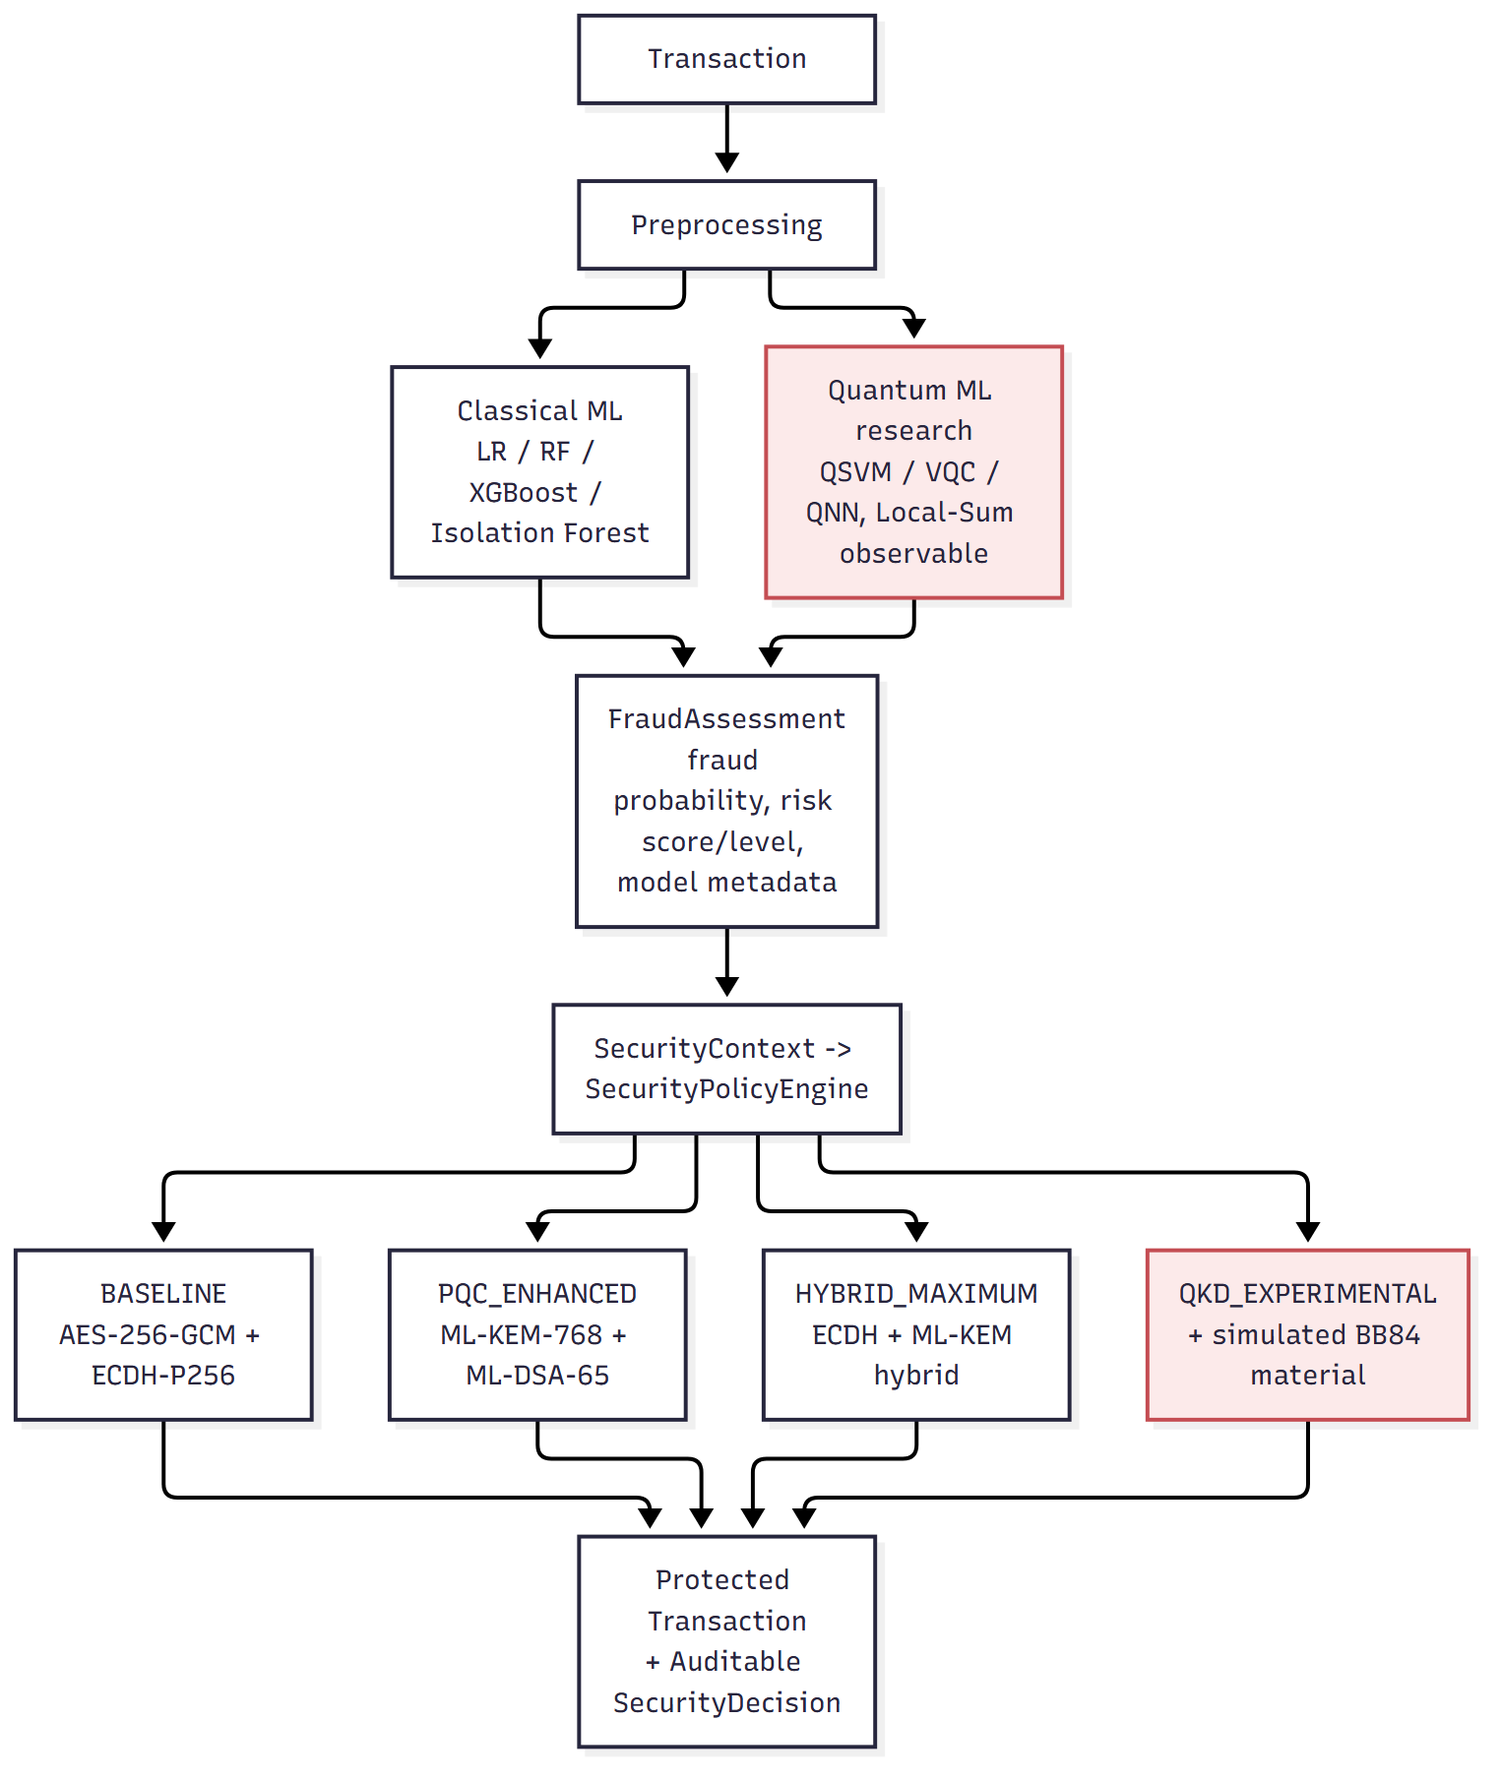
\includegraphics[width=\figw]{overall_architecture}
\caption{Overall QSFD architecture. Every security profile applies AES-256-GCM and a real key-establishment algorithm; fraud risk only selects additional protection.}
\label{fig:arch}
\end{figure}

\begin{figure}[t]
\centering
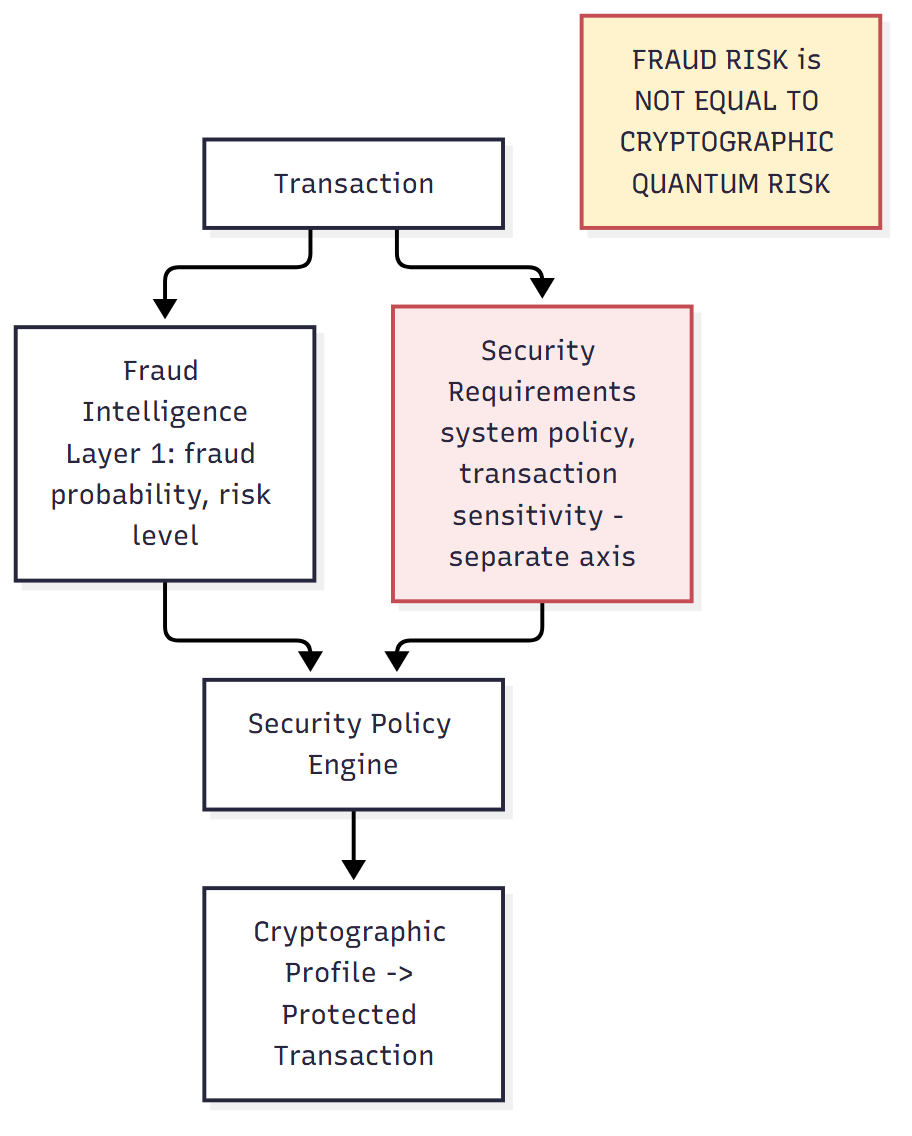
\includegraphics[width=\figw]{refined_fraud_vs_crypto_risk}
\caption{Fraud intelligence and security requirements as separate inputs to the policy engine.}
\label{fig:refined}
\end{figure}

\chapter{Implementation}
\section{Fraud Detection Methodology}\label{sec:fraud}
\subsection{Data and metrics}
Layer~1 uses the public credit-card fraud dataset~\cite{dalpozzolo} with duplicate removal before splitting, a temporal train/validation/test split, and preprocessing fitted on the training fold only. Because of the extreme imbalance, PR-AUC is the primary metric, supplemented by precision, recall and $F_1$:
\begin{equation}
\mathrm{Precision}=\frac{TP}{TP+FP},\quad
\mathrm{Recall}=\frac{TP}{TP+FN},\quad
F_1=2\,\frac{\mathrm{Precision}\cdot\mathrm{Recall}}{\mathrm{Precision}+\mathrm{Recall}}.
\label{eq:prf}
\end{equation}

\subsection{Quantum model and observable}
A classical feature vector $x$ is encoded into a parameterized state, and the model output is an expectation value:
\begin{equation}
f_\theta(x)=\langle\psi(x,\theta)|\,O\,|\psi(x,\theta)\rangle,\qquad |\psi(x,\theta)\rangle=V(\theta)\,U_{\mathrm{enc}}(x)\,|0\rangle^{\otimes n}.
\label{eq:qnn}
\end{equation}
Motivated by Cerezo et~al.~\cite{cerezo}, two observables are compared on otherwise identical circuits (Fig.~\ref{fig:obs}):
\begin{equation}
O_{\mathrm{global}}=Z_0\otimes Z_1\otimes\cdots\otimes Z_{n-1},\qquad
O_{\mathrm{local\text{-}sum}}=\frac1n\sum_{i=0}^{n-1}Z_i .
\label{eq:obs}
\end{equation}
Paired per-seed differences are $\Delta_i=\mathrm{PRAUC}^{(i)}_{\text{local-sum}}-\mathrm{PRAUC}^{(i)}_{\text{global}}$ with initialization held identical within each seed; uncertainty uses a 5000-resample bootstrap~\cite{efron}, a one-sided Wilcoxon signed-rank test~\cite{wilcoxon} and a sign-flip permutation test. The result is then tested against a matched classical nonlinear control so that quantum design effects are not conflated with added model capacity.

\begin{figure}[t]
\centering
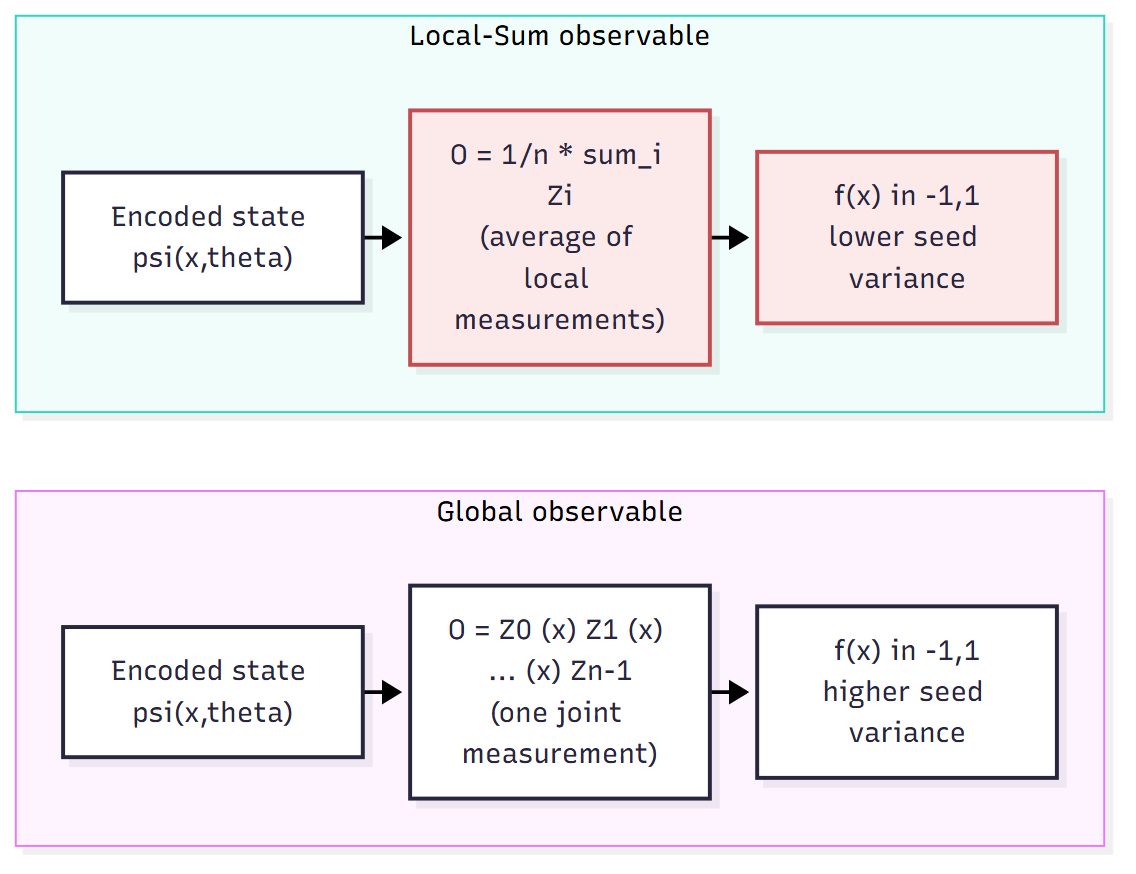
\includegraphics[width=\figw]{global_vs_localsum_diagram}
\caption{Global versus local-sum measurement on the same encoded state; only the observable differs.}
\label{fig:obs}
\end{figure}

\section{Quantum-Secure Transaction Protection}\label{sec:security}
\subsection{Primitives and roles}
Different primitives serve different functions and are compared only within a role. \emph{Bulk encryption}: AES-256-GCM in every configuration. \emph{Key establishment}: ECDH-P256 or RSA-3072 key wrap (classical) versus ML-KEM-512/768/1024 (post-quantum), following the generic KEM interface
\begin{equation}
(pk,sk)\leftarrow\mathrm{KeyGen}();\quad (c,K)\leftarrow\mathrm{Encaps}(pk);\quad K'\leftarrow\mathrm{Decaps}(sk,c);\quad K=K'.
\label{eq:kem}
\end{equation}
\emph{Signatures}: ECDSA-P256 or RSA-3072-PSS versus ML-DSA-44/65/87 and SLH-DSA-SHA2-128s/128f, with $\sigma\leftarrow\mathrm{Sign}(sk,m)$ and $\mathrm{Verify}(pk,m,\sigma)\in\{\text{true},\text{false}\}$. The hybrid profile derives the session key as
\begin{equation}
K=\mathrm{HKDF\text{-}SHA256}\bigl(K_{\mathrm{ECDH}}\,\Vert\,K_{\mathrm{ML\text{-}KEM}}\bigr).
\label{eq:hybrid}
\end{equation}

\subsection{Reference and compiled backends}
The reference implementations are pure Python (\texttt{kyber-py}, \texttt{dilithium-py}, \texttt{slh-dsa}); the compiled backend is \texttt{pqcrypto}~\cite{pqcrypto} version \PqcryptoVersion{}. Native \texttt{liboqs}~\cite{liboqs} was attempted first, but the build required CMake and an MSVC toolchain that were not present, so \emph{no liboqs measurements exist}. Both backends expose the same parameter sets and produced identical key, ciphertext and signature sizes, and a unified interface records the backend name with every measurement. Backend speedup is
\begin{equation}
S=\frac{T_{\mathrm{reference}}}{T_{\mathrm{optimized}}},\qquad
R=\frac{T_{\mathrm{reference}}-T_{\mathrm{optimized}}}{T_{\mathrm{reference}}}\times100\%,
\label{eq:speedup}
\end{equation}
which compares implementations and says nothing about cryptographic strength.

\subsection{BB84 at two simulation levels}
Alice encodes bit $a_i$ in basis $A_i\in\{Z,X\}$ as $|0\rangle,|1\rangle$ (Z) or $|\pm\rangle=(|0\rangle\pm|1\rangle)/\sqrt2$ (X); Bob measures in a random basis, and matching-basis positions form the sifted key:
\begin{equation}
Q=\frac{N_{\mathrm{error}}}{N_{\mathrm{sifted}}},\qquad
\eta_{\mathrm{sift}}=\frac{N_{\mathrm{sifted}}}{N_{\mathrm{transmitted}}}.
\label{eq:qber}
\end{equation}
The \emph{protocol-level simulator} samples basis and error outcomes directly. The \emph{Qiskit/Aer simulator} builds explicit single-qubit circuits (identity or X, then H for X-basis states; H before measurement for X-basis readout) and models noise as bit-flips after single-qubit gates. For a random-basis intercept--resend attacker, Eve's basis differs from Alice's half the time and then corrupts Bob's matched-basis outcome half the time, so ideally $Q=\tfrac12\cdot\tfrac12=25\%$. A simplified asymptotic secret fraction $\eta_{\mathrm{sift}}[1-2h_2(Q)]$ with $h_2(Q)=-Q\log_2Q-(1-Q)\log_2(1-Q)$ is reported only as a theoretical estimate, not as a finite-key bound or physical throughput. Both implementations are software simulations.

\begin{figure}[t]
\centering
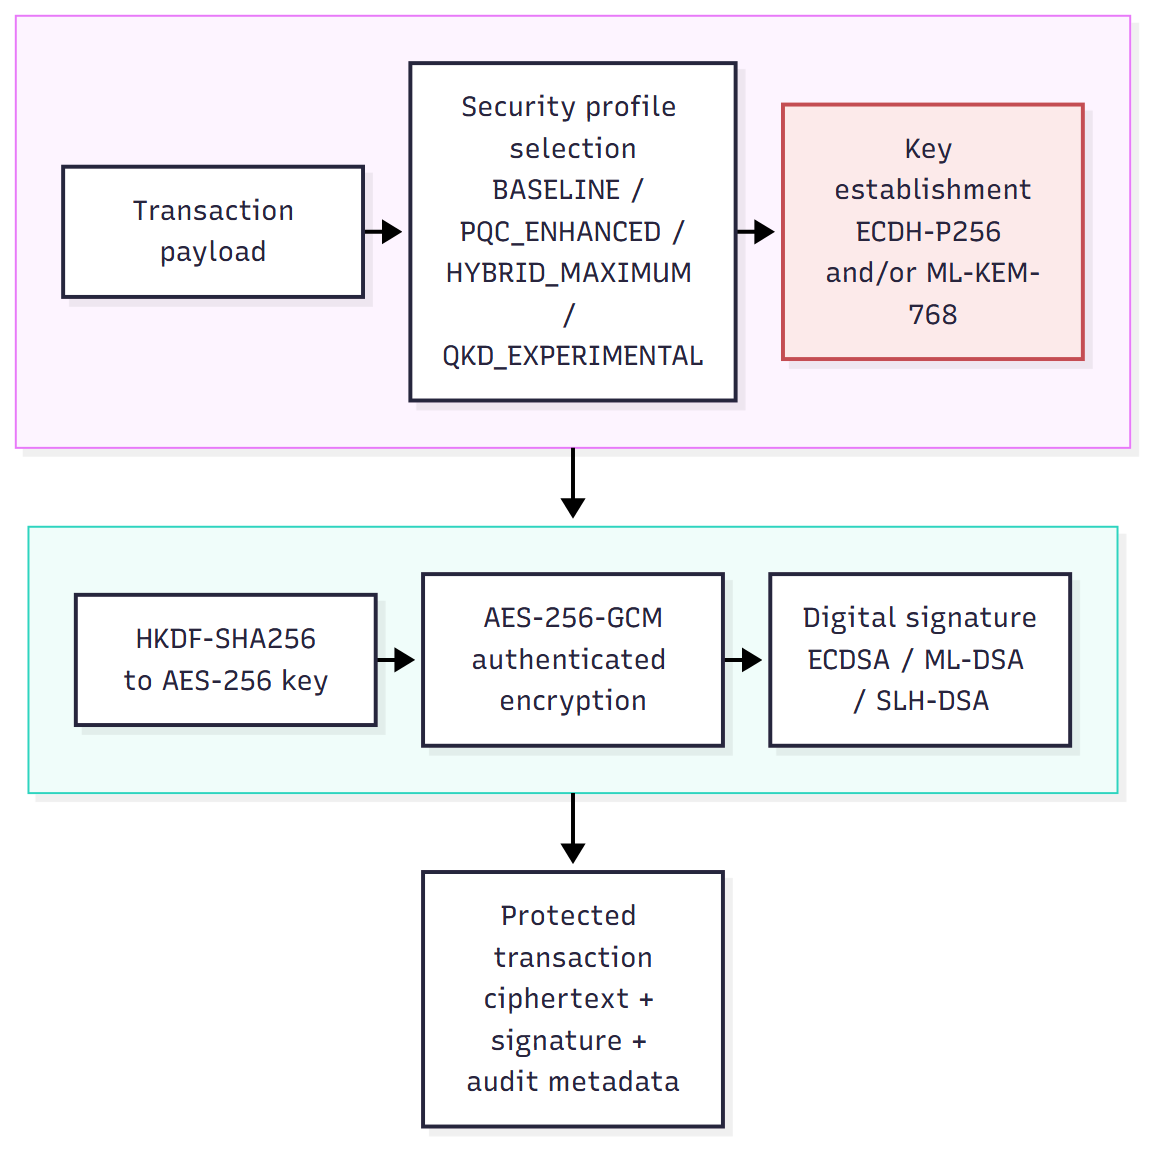
\includegraphics[width=\figw]{layer2_crypto_workflow}
\caption{Layer~2 cryptographic workflow. The KEM establishes a key; AES-256-GCM encrypts the payload.}
\label{fig:l2flow}
\end{figure}

\begin{figure}[t]
\centering
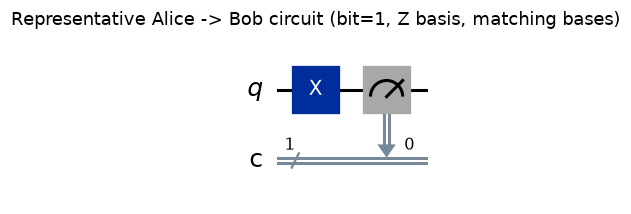
\includegraphics[width=\figw]{bb84_circuit_full_representative}
\caption{Executable Qiskit circuit for a matched-basis BB84 trial (bit 1, Z basis); circuits are generated from the project's implementation.}
\label{fig:bb84circ}
\end{figure}

\section{IBM Quantum Hardware Experimental Validation (Implementation)}
Hardware experiments were chosen only where physical execution answers a question that simulation cannot: how far real-device behaviour departs from ideal and backend-derived noisy simulation for the project's quantum components. The single-qubit BB84 preparation and measurement circuits and the intercept--resend circuit model are small enough to run on current hardware, and they connect directly to Layer~2; a two-qubit Grover circuit shows the effect of two-qubit gates. The backend was \HwBackend{} (pilot job \HwPilotJob{}, then \HwJobs{} independent jobs of 52 circuits at \HwShots{} shots). The scripts \texttt{scripts/ibm\_quantum/run\_hardware\_campaign.py} (submission), \texttt{run\_aer\_controls.py} (ideal and noisy Aer controls with the same transpiled circuits) and \texttt{analyze\_campaign.py} (analysis from saved files only) implement the study; credentials are read from a gitignored environment file and never stored. Qubits were selected from the calibration snapshot by a fixed rule before any job ran, and the snapshot, raw counts, job identifiers and transpilation statistics are saved under \texttt{results/ibm\_quantum/}. Results are given in the chapter \emph{IBM Quantum Hardware Experimental Validation}.

\chapter{Experimental Methodology}
\section{Experimental Methodology}\label{sec:method}
\paragraph{Environment.} Experiments ran on Windows~11 with Python~3.14, Qiskit~2.5.2, Qiskit~Aer~0.17.2 and \texttt{pqcrypto}~\PqcryptoVersion{} (full metadata in \texttt{results/layer2/pqc\_benchmark\_meta.json} and \texttt{results/final/final\_results.json}).

\paragraph{PQC benchmarking.} Timing used \texttt{time.perf\_counter\_ns} with warm-up runs; import and file-writing time were excluded. Compiled operations used 200 repetitions (30 for SLH-DSA-128s key generation and signing); reference operations used 30 repetitions, except reference SLH-DSA key generation and signing (3) and verification (10), because a single reference SLH-DSA signature takes seconds. Repetition counts are therefore unequal and always reported. Statistics: mean, median, standard deviation, minimum, maximum, P5, P95 and a $t$-based 95\% interval.

\paragraph{End-to-end pipeline.} A canonical JSON transaction is hashed, signed, protected with a derived session key and AES-256-GCM, passed in memory, decrypted and verified. Configurations: classical (A); reference ML-KEM-768 + ML-DSA-65 (B); compiled ML-KEM-768 + ML-DSA-65 (C); hybrid ECDH + ML-KEM with ECDSA + ML-DSA (D); and SLH-DSA-128s variants of B and C.

\paragraph{BB84.} Protocol simulator: 100 trials per condition at 500 and at 2000 transmitted bits (seeds 20000+trial). Qiskit/Aer: 50 trials per condition at 500 bits (seeds 30000+trial). Conditions: clean, 1\%, 5\% and 10\% noise, intercept--resend, and intercept--resend with 2\% noise. QBER is computed over the full sifted key. Agreement is summarized by mean absolute error, root-mean-square error and the maximum absolute difference of mean QBER, not by correlation. Detection thresholds from 0 to 0.40 are swept, treating Eve-absent trials as negatives (two noise ranges) and Eve-present trials as positives.

\paragraph{IBM Quantum hardware.} A pilot job on \HwBackend{} (17 circuits, 1024 shots) preceded a replicated campaign of \HwJobs{} independent jobs with \HwShots{} shots per circuit. The qubit-selection rule was fixed from the calibration snapshot before any job: score $=$ readout error $+$ single-qubit gate error among qubits with reported T1, T2, readout and gate errors and readout error $\le 0.2$; the \emph{best} qubit has the lowest score, the \emph{typical} qubit the median rank and the \emph{worse} qubit the 90th percentile. Each job contained matched, mismatched and intercept--resend-model BB84 circuits on each qubit and a two-qubit Grover circuit at optimization levels 0--3 on the best-calibrated coupled pair. Ideal and backend-derived noisy Aer controls used the same mappings and transpiler seed with 8192 shots; the noisy model used backend properties at analysis time. All raw counts, job IDs and calibration snapshots are stored under \texttt{results/ibm\_quantum/}; analysis runs on saved files only. Statistics: mean, standard deviation and $t$-interval over jobs, paired bootstrap and exact sign-flip permutation across jobs (with $n=5$ the smallest attainable one-sided $p$ is $1/32$, so effect sizes and intervals are primary).

\paragraph{Reproducibility.} Authoritative values live in \texttt{results/final/final\_results.json}, generated from the saved artifacts; all LaTeX numbers here are macros generated from it. The test suite has \TestsTotal{} tests (\TestsPassed{} passed, \TestsFailed{} failed, \TestsSkipped{} skipped). Commands: \texttt{python scripts/security/run\_pqc\_backend\_benchmarks.py}, \texttt{run\_end\_to\_end\_banking.py}, \texttt{run\_bb84\_final.py}, \texttt{python scripts/ibm\_quantum/analyze\_campaign.py A}, \texttt{python scripts/final/build\_final\_results.py}.

\chapter{Results and Analysis}
\section{Layer~1 Results}\label{sec:fraudres}
Among classical models, random forest reached PR-AUC \ClsRfPr{} and XGBoost \ClsXgbPr{} (logistic regression \ClsLrPr{}; isolation forest \ClsIfPr{}). XGBoost was retained for production because of much lower latency at a similar PR-AUC, not because of the highest point estimate.

In the decisive quantum experiment (\LsSeeds{} paired seeds), the local-sum observable improved PR-AUC over the global observable by a mean of \LsDelta{} (bootstrap 95\% CI [\LsCIlo{}, \LsCIhi{}]; one-sided Wilcoxon $p=\LsWilcoxon{}$; permutation $p=\LsPerm{}$; local-sum better in \LsWins{} of \LsSeeds{} seeds). Fig.~\ref{fig:paired} shows the paired per-seed comparison. This supports an architecture-level effect of observable choice. It does \emph{not} establish a system-level quantum advantage: on the locked confirmation split, XGBoost alone scored \CapXgb{}, XGBoost plus the local-sum QNN \CapXgbLocal{}, and XGBoost plus a matched classical control \CapXgbControl{}; the bootstrap CI of the quantum increment over XGBoost alone, [\CapCIlo{}, \CapCIhi{}], includes zero. Every other quantum configuration evaluated (QSVM, VQC, Chow--Liu circuits, QBoost, hybrid fusion architectures, quantum-kernel anomaly detection at scale) likewise failed to beat its classical counterpart; these negative results are retained in the repository.

\begin{figure}[t]
\centering
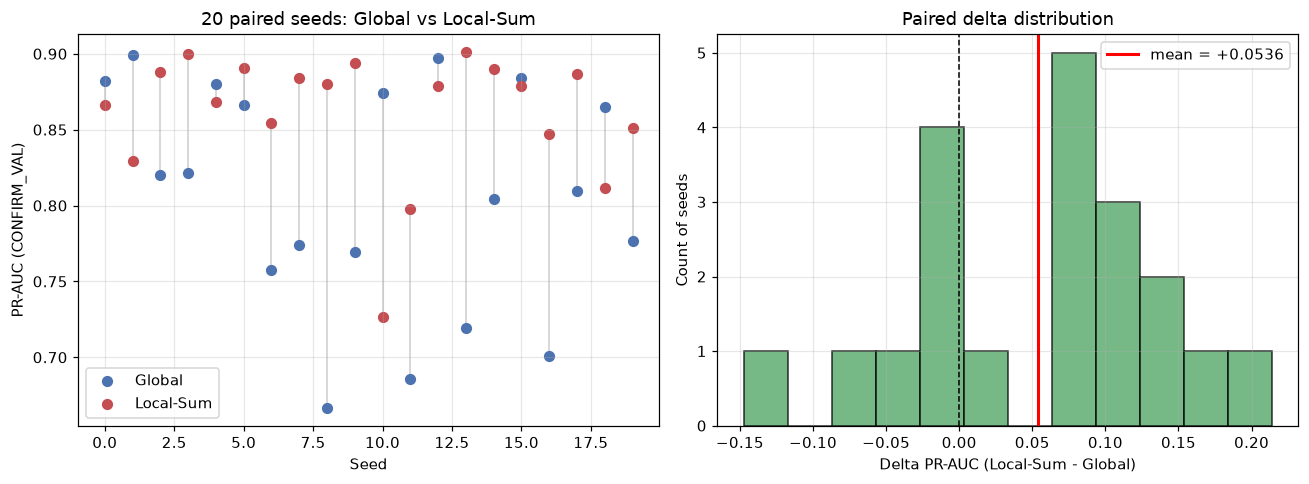
\includegraphics[width=\figw]{paired_seed_deltas}
\caption{Paired PR-AUC comparison of the global and local-sum QNN across matched seeds.}
\label{fig:paired}
\end{figure}

\section{Layer~2 Results}\label{sec:l2res}
\subsection{Reference versus compiled PQC}
Table~\ref{tab:pqc-comparison} compares median latencies. Over all compared operations the speedup ranged from \SpeedupMin{}$\times$ to \SpeedupMax{}$\times$. ML-KEM-768 key generation, encapsulation and decapsulation were \SpeedupMlkemKeygen{}$\times$, \SpeedupMlkemEncaps{}$\times$ and \SpeedupMlkemDecaps{}$\times$ faster with the compiled backend, and ML-DSA-65 key generation and verification were \SpeedupMldsaKeygen{}$\times$ and \SpeedupMldsaVerify{}$\times$ faster, i.e.\ these costs are strongly implementation-dependent. ML-DSA-65 signing improved only \SpeedupMldsaSign{}$\times$ (median \RefMldsaSignMs{}~ms to \OptMldsaSignMs{}~ms), consistent with the variable-iteration rejection sampling in its signing procedure.

\begin{table}[t]
\centering
\small
\caption{Reference Python vs.\ \texttt{pqcrypto}: median latency and implementation-backend speedup (selected parameter sets). $n$ is the number of timed repetitions.}
\label{tab:pqc-comparison}
\resizebox{\linewidth}{!}{%
\begin{tabular}{llrrrrr}
\toprule
Algorithm & Op. & n ref & n opt & Ref. median (ms) & pqcrypto median (ms) & Speedup \\
\midrule
ML-DSA-65 & keygen & 30 & 200 & 11.5 & 0.237 & 48.5 \\
ML-DSA-65 & sign & 30 & 200 & 45.5 & 9.45 & 4.81 \\
ML-DSA-65 & verify & 30 & 200 & 12.7 & 0.22 & 57.6 \\
ML-KEM-768 & decaps & 30 & 200 & 6.78 & 0.111 & 61 \\
ML-KEM-768 & encaps & 30 & 200 & 5.02 & 0.0876 & 57.3 \\
ML-KEM-768 & keygen & 30 & 200 & 3.71 & 0.0721 & 51.5 \\
SLH-DSA-SHA2-128f & keygen & 3 & 200 & 22.8 & 2.56 & 8.94 \\
SLH-DSA-SHA2-128f & sign & 3 & 200 & 231 & 60.2 & 3.84 \\
SLH-DSA-SHA2-128f & verify & 10 & 200 & 12.8 & 3.68 & 3.47 \\
SLH-DSA-SHA2-128s & keygen & 3 & 30 & 1.25e+03 & 163 & 7.69 \\
SLH-DSA-SHA2-128s & sign & 3 & 30 & 4.33e+03 & 1.27e+03 & 3.41 \\
SLH-DSA-SHA2-128s & verify & 10 & 200 & 4.42 & 1.23 & 3.59 \\
\bottomrule
\end{tabular}}
\end{table}


\paragraph{The SLH-DSA question.} An earlier session measured about 15~s per SLH-DSA-SHA2-128s signature with the reference code (n=5); that value is preserved. In the controlled run reported here, the reference median was \RefSlhSSignMs{}~ms (n=\SlhSRefN{}) and the compiled median \OptSlhSSignMs{}~ms (n=\SlhSOptN{}), a \SpeedupSlhSSign{}$\times$ difference, and the fast variant 128f signed in \OptSlhFSignMs{}~ms compiled. Two conclusions follow. First, the ${\sim}15$~s figure is reference-implementation behaviour from a different session and is not an implementation-independent property. Second, compiled SLH-DSA-128s signing remains about two orders of magnitude slower than compiled ML-DSA-65 (\OptMldsaSignMs{}~ms), so most of its signing cost is a property of the parameter set rather than only of the implementation.

\begin{figure}[t]
\centering
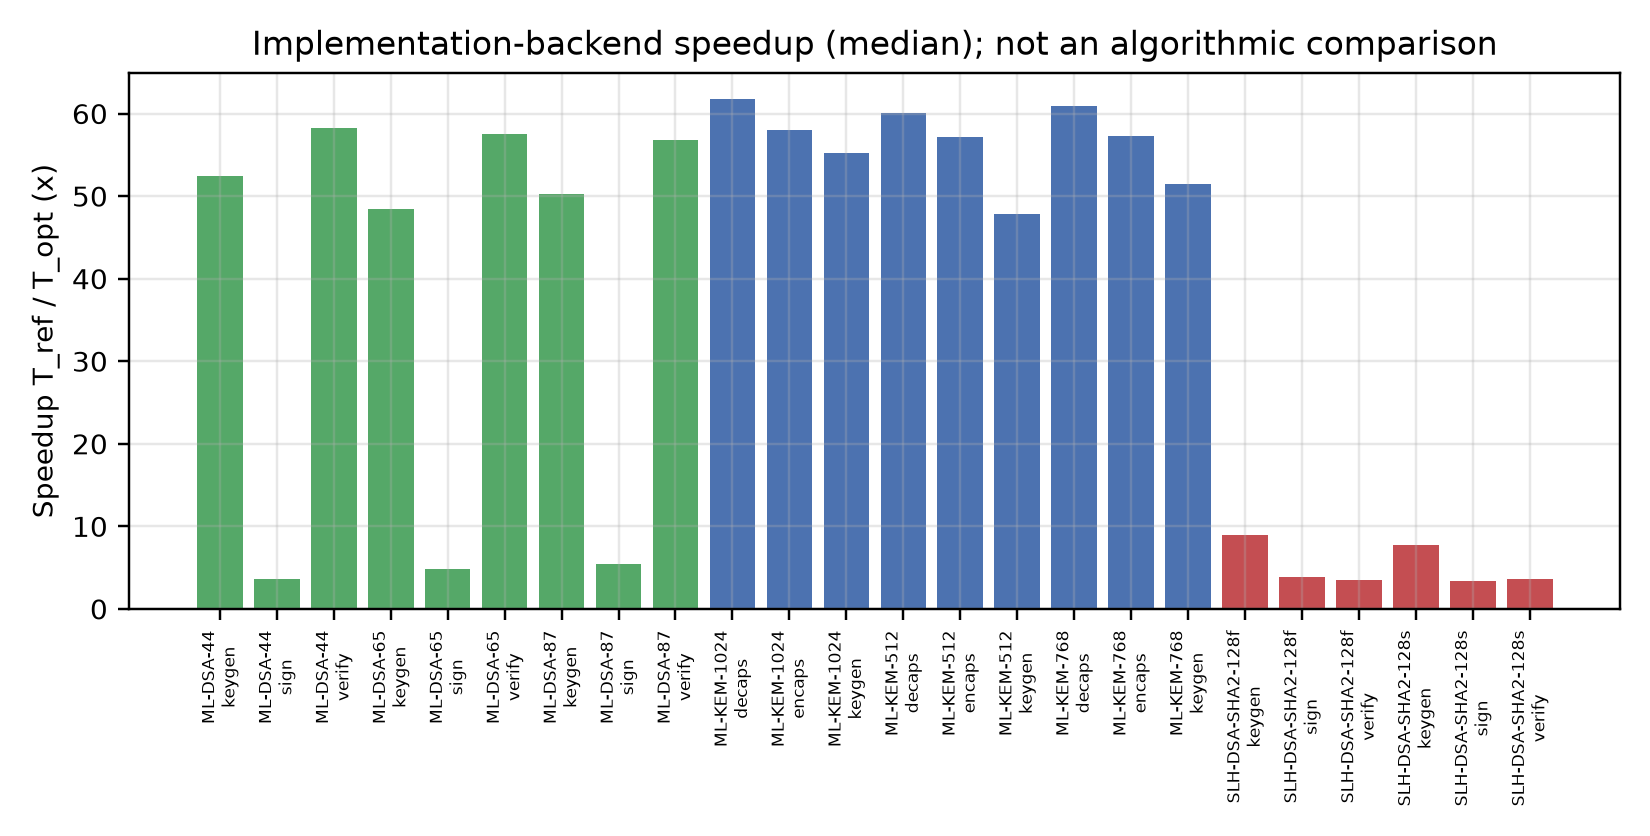
\includegraphics[width=\figw]{pqc_backend_speedup}
\caption{Implementation-backend speedup per operation (median ratio). This compares implementations, not cryptographic strength.}
\label{fig:speedup}
\end{figure}
\begin{figure}[t]
\centering
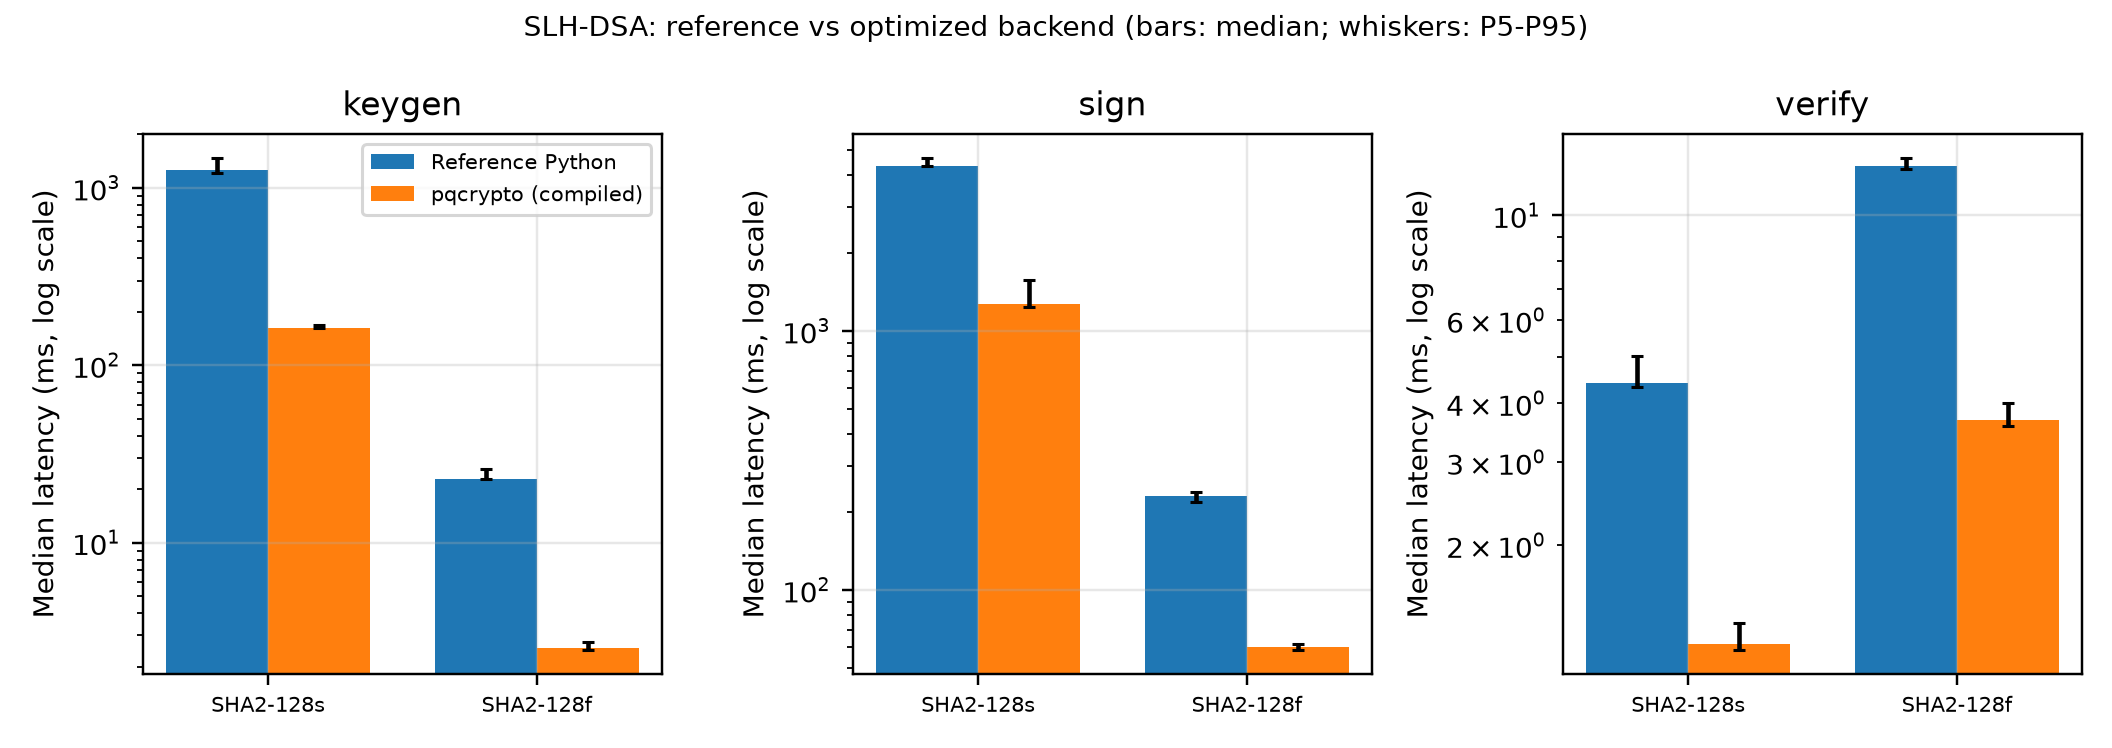
\includegraphics[width=\figw]{pqc_ref_vs_opt_slhdsa}
\caption{SLH-DSA reference versus compiled latency (log-scale; reference signing $n=3$).}
\label{fig:slh}
\end{figure}
\begin{figure}[t]
\centering
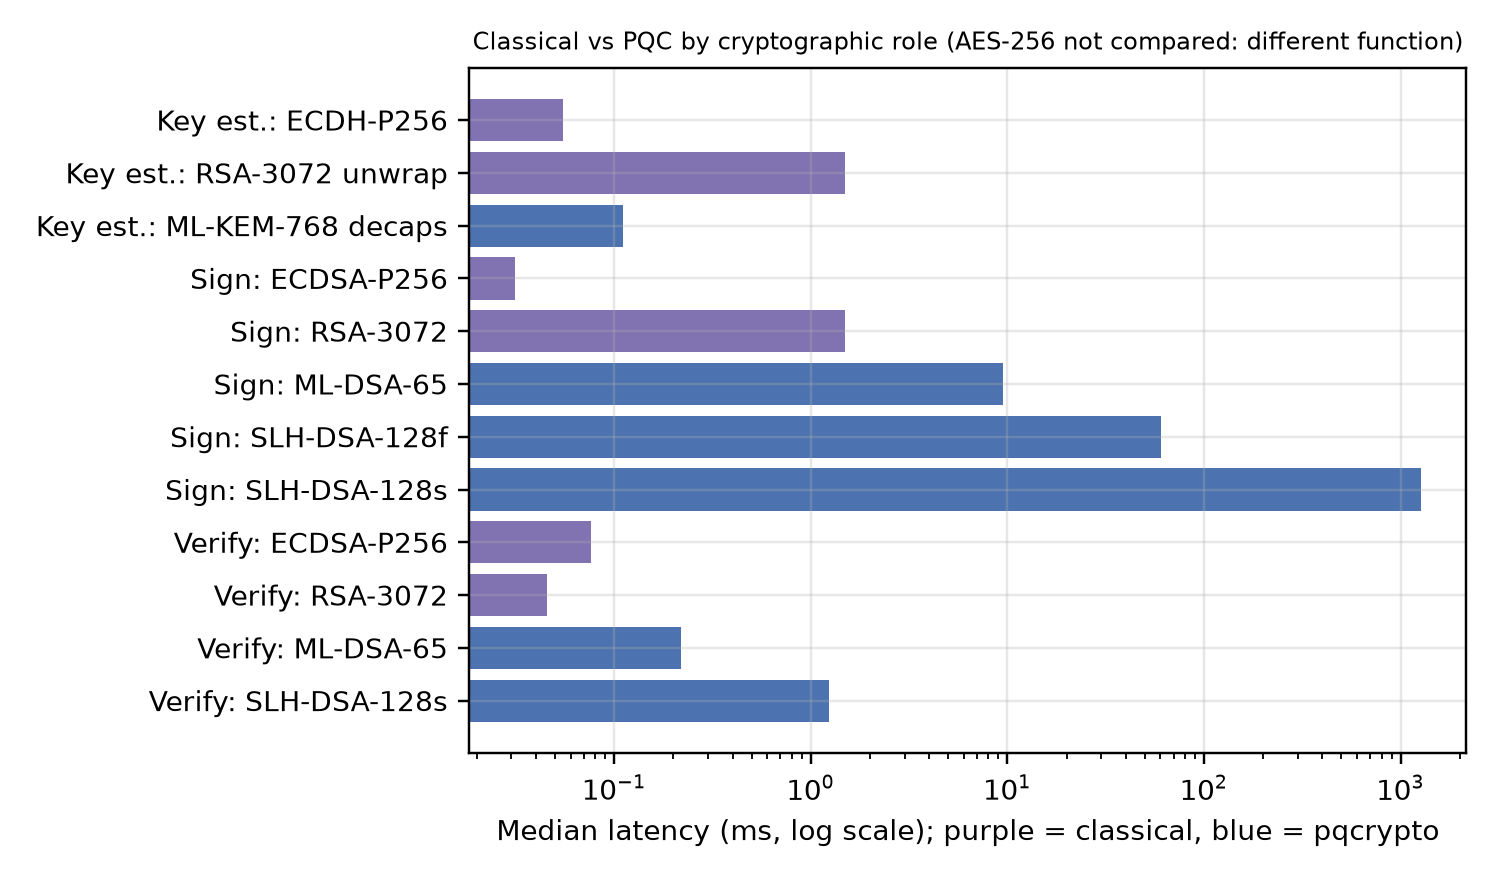
\includegraphics[width=\figw]{classical_vs_pqc_latency}
\caption{Median latency by cryptographic role, classical versus post-quantum (log-scale). AES-256 is excluded because it performs a different function.}
\label{fig:classical}
\end{figure}
\begin{figure}[t]
\centering
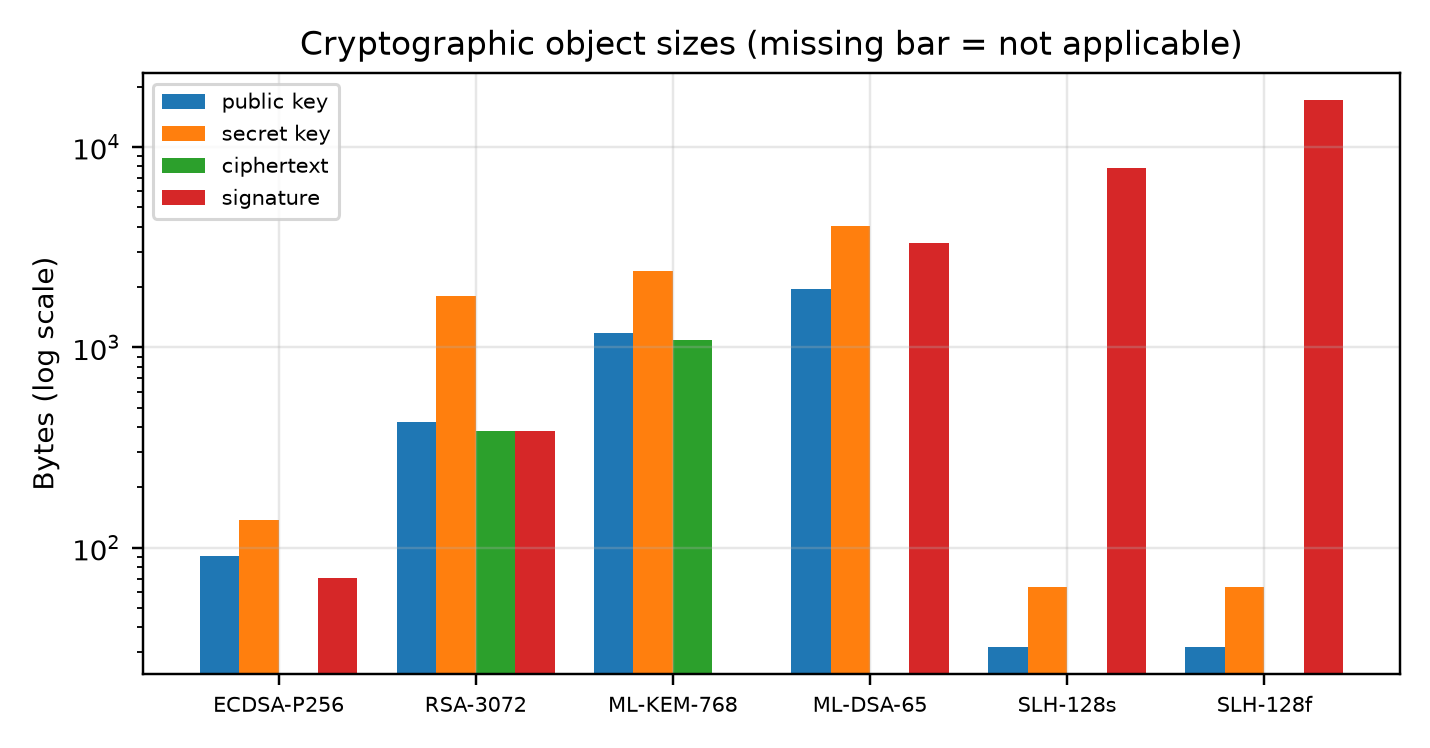
\includegraphics[width=\figw]{crypto_object_sizes}
\caption{Key, ciphertext and signature sizes (log-scale; missing bar means not applicable). Sizes are identical across the two PQC backends.}
\label{fig:sizes}
\end{figure}

\subsection{End-to-end banking-transaction protection}
Table~\ref{tab:e2e} gives total latency including serialization, signing, key establishment, encryption, decryption and verification. The classical configuration had a median of \EEAMedian{}~ms; compiled ML-KEM-768 + ML-DSA-65 \EECMedian{}~ms; the same with reference code \EEBMedian{}~ms; the hybrid configuration \EEDMedian{}~ms. Configurations using SLH-DSA-128s were dominated by signing (\EEBTwoMedian{}~ms reference, \EECTwoMedian{}~ms compiled). Secured payload grew to \EEAExpansion{}$\times$ the plaintext (\PlaintextBytes{}~B) classically, \EECExpansion{}$\times$ with ML-KEM/ML-DSA and \EECTwoExpansion{}$\times$ with ML-KEM/SLH-DSA, almost entirely from KEM ciphertext and signature bytes. Simulated transmission is in-memory, so no network latency is included.

\begin{table}[t]
\centering
\small
\caption{End-to-end banking-transaction protection (serialize--sign--key establishment--AES-256-GCM--decrypt--verify). Plaintext is the same canonical JSON payload in all rows.}
\label{tab:e2e}
\resizebox{\linewidth}{!}{%
\begin{tabular}{lrrrrr}
\toprule
Configuration & n & Median (ms) & P95 (ms) & Secured (B) & Expansion \\
\midrule
A\_classical\_ECDH+ECDSA & 200 & 0.302 & 0.568 & 475 & 1.52 \\
B\_reference\_ML-KEM-768+ML-DSA-65 & 30 & 72.8 & 141 & 4737 & 15.2 \\
C\_optimized\_ML-KEM-768+ML-DSA-65 & 200 & 10.2 & 11 & 4737 & 15.2 \\
D\_hybrid\_optimized\_ECDH+ML-KEM-768\_ECDSA+ML-DSA-65 & 200 & 10.5 & 11 & 4873 & 15.6 \\
B2\_reference\_ML-KEM-768+SLH-DSA-128s & 3 & 3.63e+03 & 3.66e+03 & 9284 & 29.8 \\
C2\_optimized\_ML-KEM-768+SLH-DSA-128s & 20 & 1.25e+03 & 1.27e+03 & 9284 & 29.8 \\
\bottomrule
\end{tabular}}
\end{table}


\begin{figure}[t]
\centering
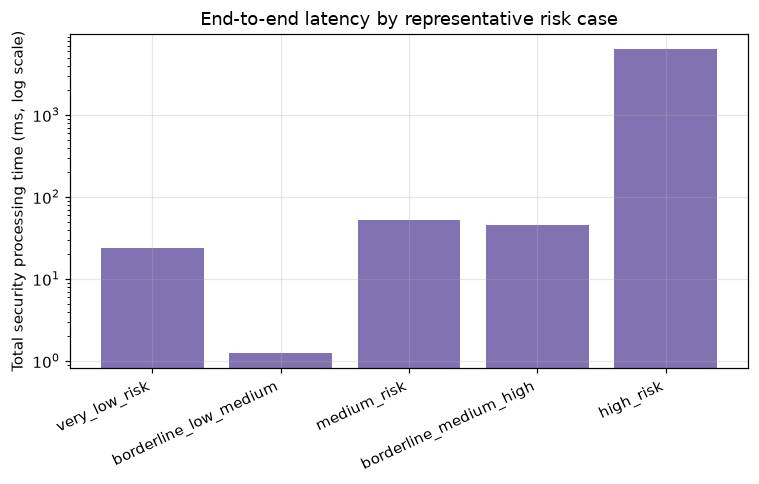
\includegraphics[width=\figw]{end_to_end_latency}
\caption{End-to-end latency by configuration (log-scale; whiskers to P95).}
\label{fig:e2e}
\end{figure}

\subsection{BB84 statistics and cross-validation}
Table~\ref{tab:bb84} and Fig.~\ref{fig:qberci} report QBER with confidence intervals. The clean channel gave QBER 0 in both implementations. With injected noise of 1\%, 5\% and 10\%, mean QBER was \BbqProtoKOnePct{}, \BbqProtoKFivePct{} and \BbqProtoKTenPct{} (protocol, 2000 bits) and \BbqQiskOnePct{}, \BbqQiskFivePct{} and \BbqQiskTenPct{} (Qiskit, 500 bits). With the intercept--resend attacker, mean QBER was \BbqProtoKEve{} (95\% CI \BbciProtoKEve{}) and \BbqQiskEve{} (95\% CI \BbciQiskEve{}) against the theoretical 0.25; adding 2\% noise raised them to \BbqProtoKEveNoise{} and \BbqQiskEveNoise{}. Both attack intervals can be read directly against 0.25 in Fig.~\ref{fig:qberci}; no value was tuned toward the theory. Comparing the two implementations at 500 bits per trial gave MAE \BbMAE{}, RMSE \BbRMSE{} and a maximum difference of \BbMaxDiff{} in mean QBER. Sifting efficiency was \SiftEff{} (theory 0.5).

\begin{table}[t]
\centering
\small
\caption{BB84 software simulation: protocol simulator (2000 bits/trial) and Qiskit/Aer circuit simulator (500 bits/trial). QBER over the full sifted key; 95\% $t$-interval over trials; detection rate = fraction of trials with QBER above 0.11.}
\label{tab:bb84}
\resizebox{\linewidth}{!}{%
\begin{tabular}{llrrrrrrr}
\toprule
Impl. & Condition & Trials & Bits & \$\textbackslash eta\_\{sift\}\$ & Mean QBER & CI low & CI high & Det. rate \\
\midrule
protocol 2000 & clean & 100 & 2000 & 0.4999 & 0.0000 & 0.0000 & 0.0000 & 0.0000 \\
protocol 2000 & noise\_1pct & 100 & 2000 & 0.4999 & 0.0097 & 0.0091 & 0.0103 & 0.0000 \\
protocol 2000 & noise\_5pct & 100 & 2000 & 0.4999 & 0.0490 & 0.0477 & 0.0504 & 0.0000 \\
protocol 2000 & noise\_10pct & 100 & 2000 & 0.4999 & 0.0979 & 0.0960 & 0.0999 & 0.1200 \\
protocol 2000 & eve\_intercept\_resend & 100 & 2000 & 0.4996 & 0.2508 & 0.2479 & 0.2537 & 1.0000 \\
protocol 2000 & eve\_and\_noise\_2pct & 100 & 2000 & 0.4996 & 0.2606 & 0.2578 & 0.2635 & 1.0000 \\
qiskit 500 & clean & 50 & 500 & 0.4991 & 0.0000 & 0.0000 & 0.0000 & 0.0000 \\
qiskit 500 & noise\_1pct & 50 & 500 & 0.4991 & 0.0082 & 0.0059 & 0.0104 & 0.0000 \\
qiskit 500 & noise\_5pct & 50 & 500 & 0.4991 & 0.0498 & 0.0458 & 0.0538 & 0.0000 \\
qiskit 500 & noise\_10pct & 50 & 500 & 0.4991 & 0.0960 & 0.0896 & 0.1023 & 0.2200 \\
qiskit 500 & eve\_intercept\_resend & 50 & 500 & 0.4991 & 0.2438 & 0.2360 & 0.2515 & 1.0000 \\
qiskit 500 & eve\_and\_noise\_2pct & 50 & 500 & 0.4991 & 0.2649 & 0.2576 & 0.2722 & 1.0000 \\
\bottomrule
\end{tabular}}
\end{table}


\begin{figure}[t]
\centering
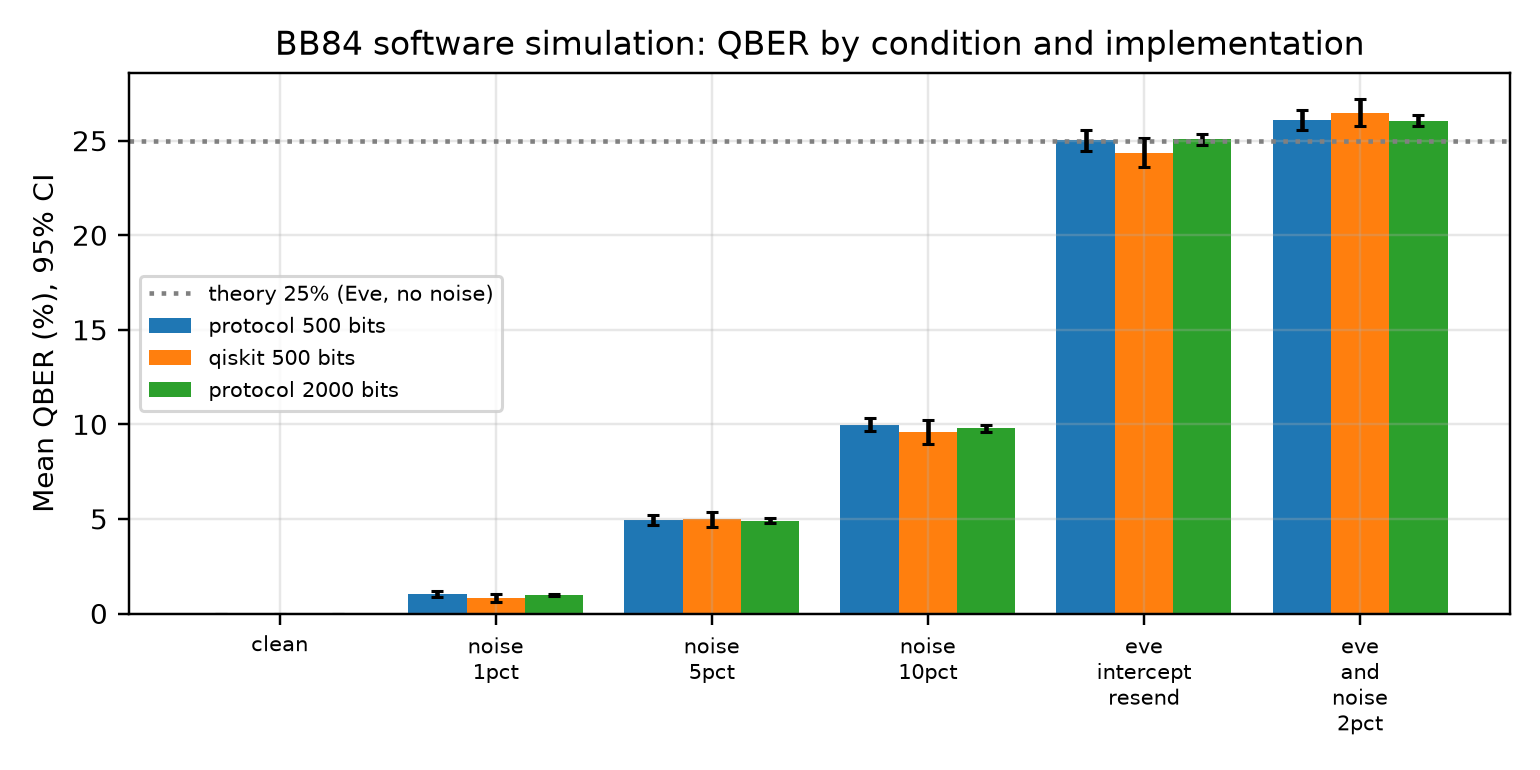
\includegraphics[width=\figw]{bb84_final_qber_ci}
\caption{Mean QBER with 95\% confidence intervals by condition and implementation; dotted line: 25\% theory for intercept--resend.}
\label{fig:qberci}
\end{figure}
\begin{figure}[t]
\centering
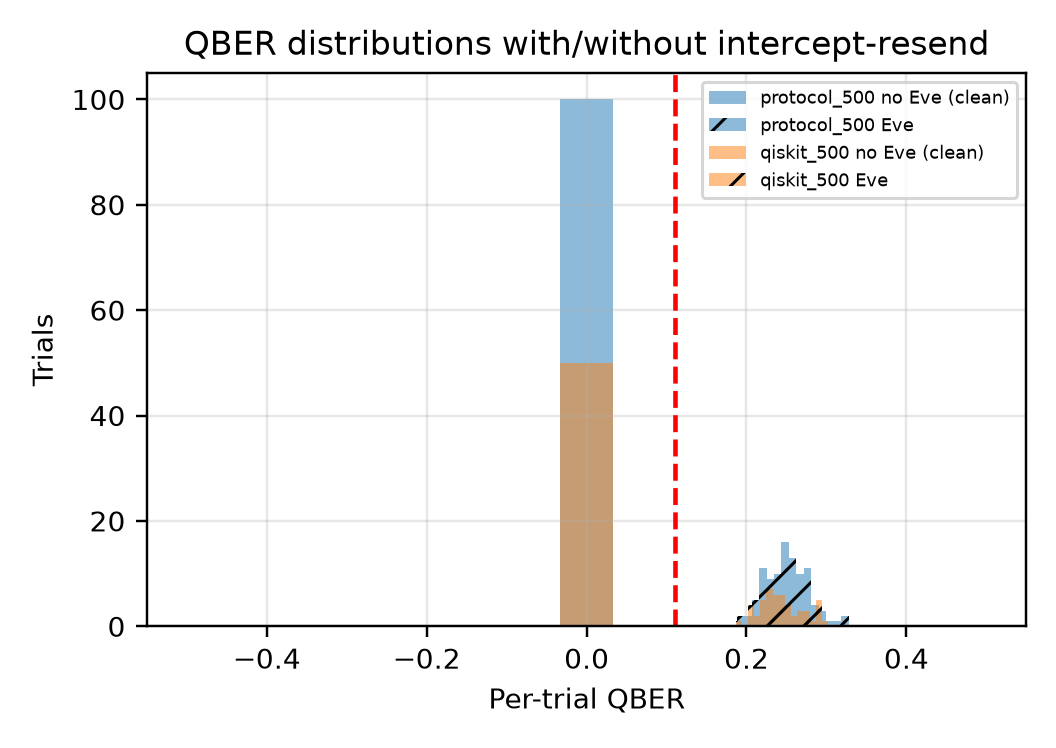
\includegraphics[width=\figw]{bb84_final_eve_distribution}
\caption{Per-trial QBER with and without intercept--resend; dashed line: 0.11 threshold.}
\label{fig:evedist}
\end{figure}

\subsection{Eve-detection threshold}
At the conventional 0.11 threshold, the true-positive rate was \ThrTPRProtoK{} (protocol, 2000 bits), \ThrTPRProtoH{} (protocol, 500 bits) and \ThrTPRQisk{} (Qiskit), while the false-positive rate when 10\%-noise trials count as Eve-absent was \ThrFPRProtoK{}, \ThrFPRProtoH{} and \ThrFPRQisk{} (Table~\ref{tab:threshold}, Fig.~\ref{fig:thr}). A higher threshold (first maximum of balanced accuracy at \ThrBestAProtoK{}, \ThrBestAProtoH{} and \ThrBestAQisk{}) separates the classes in these simulations, but that optimum depends on the noise range chosen and is not a general security threshold. QBER above a threshold does not prove eavesdropping, because channel noise also increases QBER.

\begin{table}[t]
\centering
\small
\caption{Eve-detection threshold analysis at the conventional 0.11 value; last column is the lowest threshold attaining the maximum balanced accuracy in this simulated design.}
\label{tab:threshold}
\resizebox{\linewidth}{!}{%
\begin{tabular}{llrrrr}
\toprule
Impl. & Eve-absent set & TPR@0.11 & FPR@0.11 & Miss@0.11 & First best thr. \\
\midrule
protocol 2000 & no eve all noise levels & 1.000 & 0.030 & 0.000 & 0.120 \\
protocol 2000 & no eve clean to 5pct & 1.000 & 0.000 & 0.000 & 0.070 \\
protocol 500 & no eve all noise levels & 1.000 & 0.085 & 0.000 & 0.140 \\
protocol 500 & no eve clean to 5pct & 1.000 & 0.000 & 0.000 & 0.080 \\
qiskit 500 & no eve all noise levels & 1.000 & 0.055 & 0.000 & 0.160 \\
qiskit 500 & no eve clean to 5pct & 1.000 & 0.000 & 0.000 & 0.090 \\
\bottomrule
\end{tabular}}
\end{table}


\begin{figure}[t]
\centering
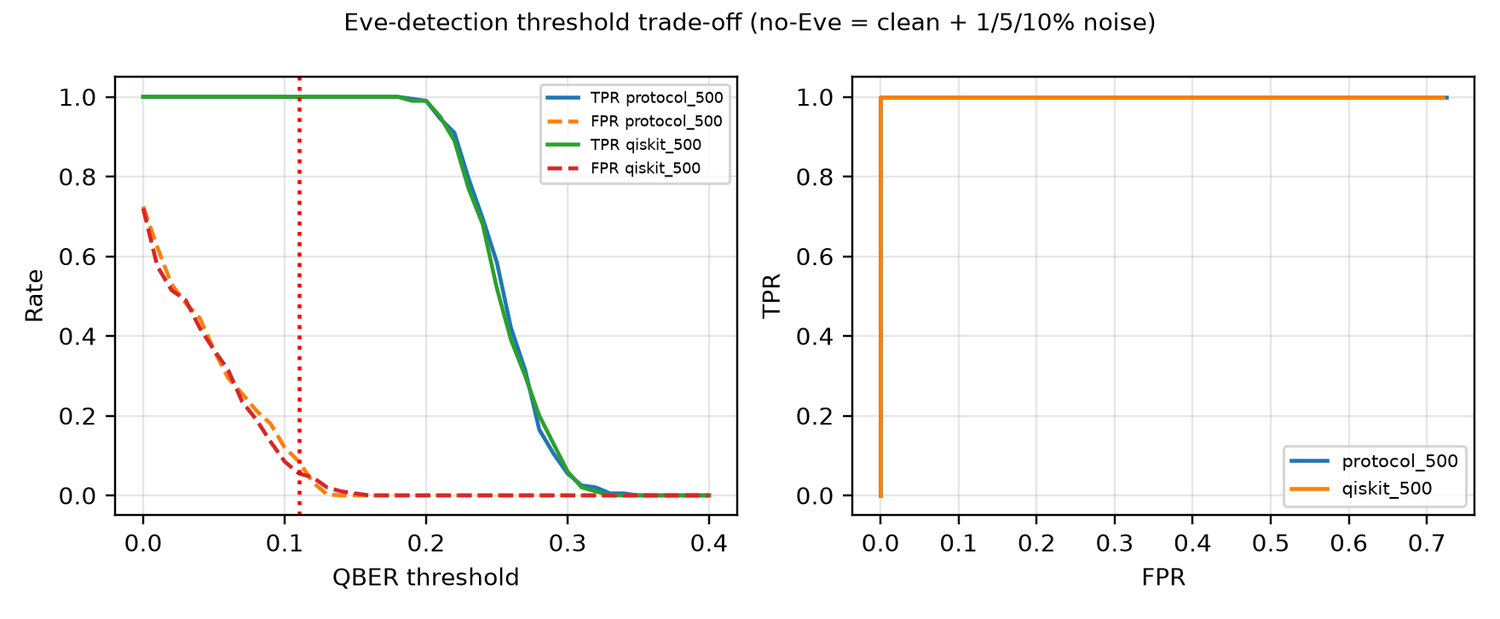
\includegraphics[width=\figw]{bb84_threshold_tradeoff}
\caption{Eve-detection threshold trade-off: TPR/FPR against threshold and ROC-style view.}
\label{fig:thr}
\end{figure}

\chapter{IBM Quantum Hardware Experimental Validation}
\section{IBM Quantum Hardware Validation}\label{sec:hw}
\subsection{Scope and provenance}
Selected QSFD circuits were executed on IBM Quantum hardware to measure how far real-device behaviour departs from ideal and backend-derived noisy simulation. The campaign used \HwBackend{} with \HwJobs{} independent jobs of 52 circuits at \HwShots{} shots each (\HwCircuits{} circuits, \HwTotalShots{} shots), after a pilot job (\HwPilotJob{}; 17 circuits, 1024 shots) that is retained as a baseline. An earlier job on \texttt{ibm\_fez} (\HwFezJob{}) executed the Layer~1 QNN circuits and is reported separately. These runs validate circuit-level components; they do not execute the full fraud classifier and are not physical quantum key distribution.

\subsection{BB84 primitives and the intercept--resend model}
Table~\ref{tab:hw-backend} compares theory, ideal Aer, noisy Aer and hardware. With no Eve, hardware QBER was \HwNoEveBest{} (95\% CI \HwNoEveCIBest{}) on the best-calibrated qubit (physical qubit \HwQubitBest{}, readout error \HwReadoutBest{}), \HwNoEveTypical{} on the typical qubit and \HwNoEveWorse{} on the worse qubit (readout error \HwReadoutWorse{}); the ordering matches the readout-error ordering, although with three qubits only a descriptive comparison is made. The intercept--resend circuit model raised QBER to \HwEveBest{}, \HwEveTypical{} and \HwEveWorse{}, i.e.\ by \HwDeltaBest{}, \HwDeltaTypical{} and \HwDeltaWorse{} relative to no Eve (paired bootstrap CI for the best qubit [\HwDeltaBootLoBest{}, \HwDeltaBootHiBest{}]; exact sign-flip permutation $p=\HwPermBest{}$, the minimum attainable with five pairs). Attack-induced error stayed separable from hardware error in every job and qubit cell: the largest no-Eve QBER (\HwMaxNoEve{}) was below the smallest Eve QBER (\HwMinEve{}). The ideal expectation of 25\% is a reference rather than a pass/fail target; hardware values above it are consistent with hardware-induced error added to attack-induced error.

\begin{table}[t]
\centering
\small
\caption{Theory vs.\ ideal Aer vs.\ backend-derived noisy Aer vs.\ IBM hardware (ibm\_marrakesh); mean and 95\% $t$-interval over independent jobs.}
\label{tab:hw-backend}
\resizebox{\linewidth}{!}{%
\begin{tabular}{llrrrrrrr}
\toprule
Experiment & Qubit & Theory & Ideal Aer & Noisy Aer & IBM mean & CI low & CI high & Jobs \\
\midrule
BB84 matched-basis QBER (no Eve) & best (q98) & 0.0000 & 0.0000 & 0.0025 & 0.0048 & 0.0036 & 0.0060 & 5 \\
Intercept-resend QBER & best (q98) & 0.2500 & 0.2500 & 0.2512 & 0.2632 & 0.2579 & 0.2685 & 5 \\
BB84 matched-basis QBER (no Eve) & typical (q155) & 0.0000 & 0.0000 & 0.0110 & 0.0094 & 0.0082 & 0.0106 & 5 \\
Intercept-resend QBER & typical (q155) & 0.2500 & 0.2500 & 0.2557 & 0.2591 & 0.2535 & 0.2648 & 5 \\
BB84 matched-basis QBER (no Eve) & worse (q126) & 0.0000 & 0.0000 & 0.0738 & 0.0446 & 0.0277 & 0.0616 & 5 \\
Intercept-resend QBER & worse (q126) & 0.2500 & 0.2500 & 0.2873 & 0.2868 & 0.2796 & 0.2939 & 5 \\
Grover 2q success probability & pair [135, 139] & 1.0000 & 1.0000 & 0.9678 & 0.9460 & 0.9386 & 0.9534 & 5 \\
\bottomrule
\end{tabular}}
\end{table}

\begin{table}[t]
\centering
\small
\caption{Physical qubits used and their calibration snapshot at campaign start, with observed hardware error.}
\label{tab:hw-calibration}
\resizebox{\linewidth}{!}{%
\begin{tabular}{lrrrrrlr}
\toprule
Role & Qubit & T1 (\$\textbackslash mu\$s) & T2 (\$\textbackslash mu\$s) & Readout err. & 1Q err. & Circuit & No-Eve QBER \\
\midrule
best & 98 & 265.6 & 68.85 & 0.002075 & 0.0008155 & BB84 single-qubit & 0.004785 \\
typical & 155 & 393.9 & 107 & 0.01221 & 0.0003537 & BB84 single-qubit & 0.009399 \\
worse & 126 & 104.3 & 8.646 & 0.07593 & 0.0004358 & BB84 single-qubit & 0.04463 \\
grover\_pair & 135 & 294.5 & 91.06 & 0.02295 & 0.0001081 & Grover 2q (cz err 0.0011) & -- \\
grover\_pair & 139 & 136.3 & 158.9 & 0.005371 & 0.00019 & Grover 2q (cz err 0.0011) & -- \\
\bottomrule
\end{tabular}}
\end{table}


\begin{figure}[t]
\centering
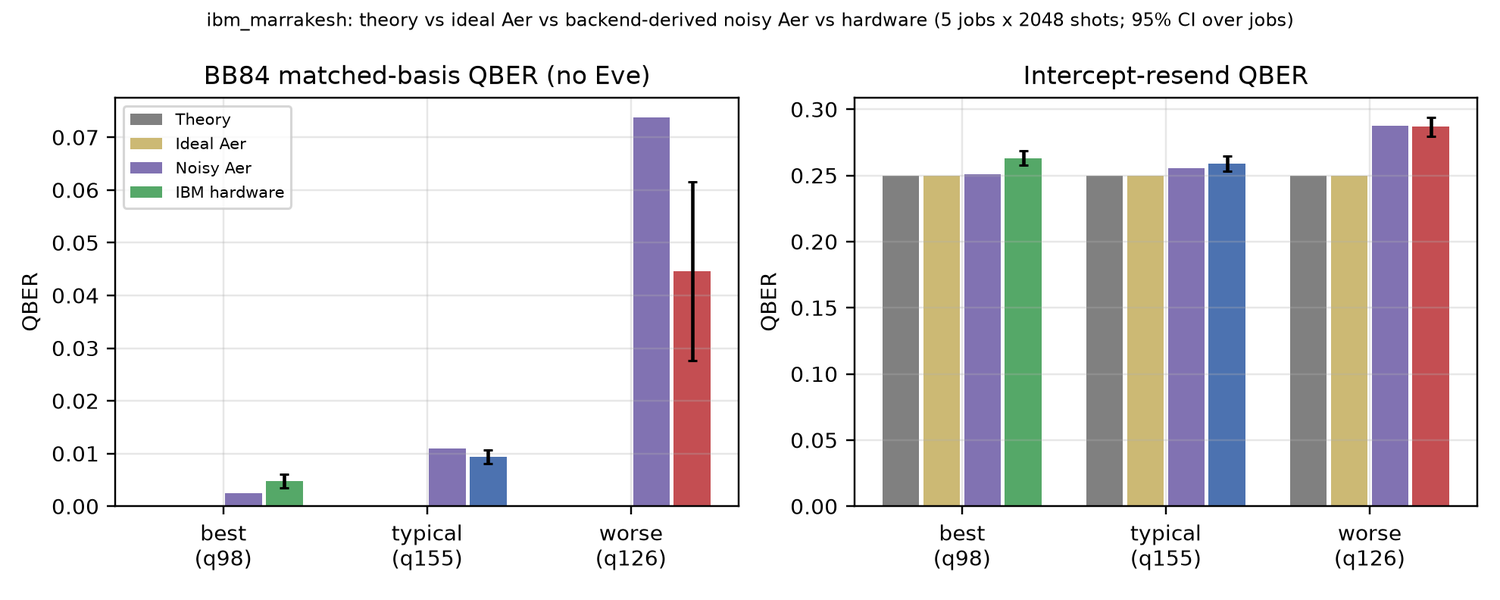
\includegraphics[width=\figw]{hw_qber_theory_ideal_noisy_hardware}
\caption{BB84 QBER: theory, ideal Aer, backend-derived noisy Aer and IBM hardware (95\% CI over independent jobs).}
\label{fig:hwqber}
\end{figure}
\begin{figure}[t]
\centering
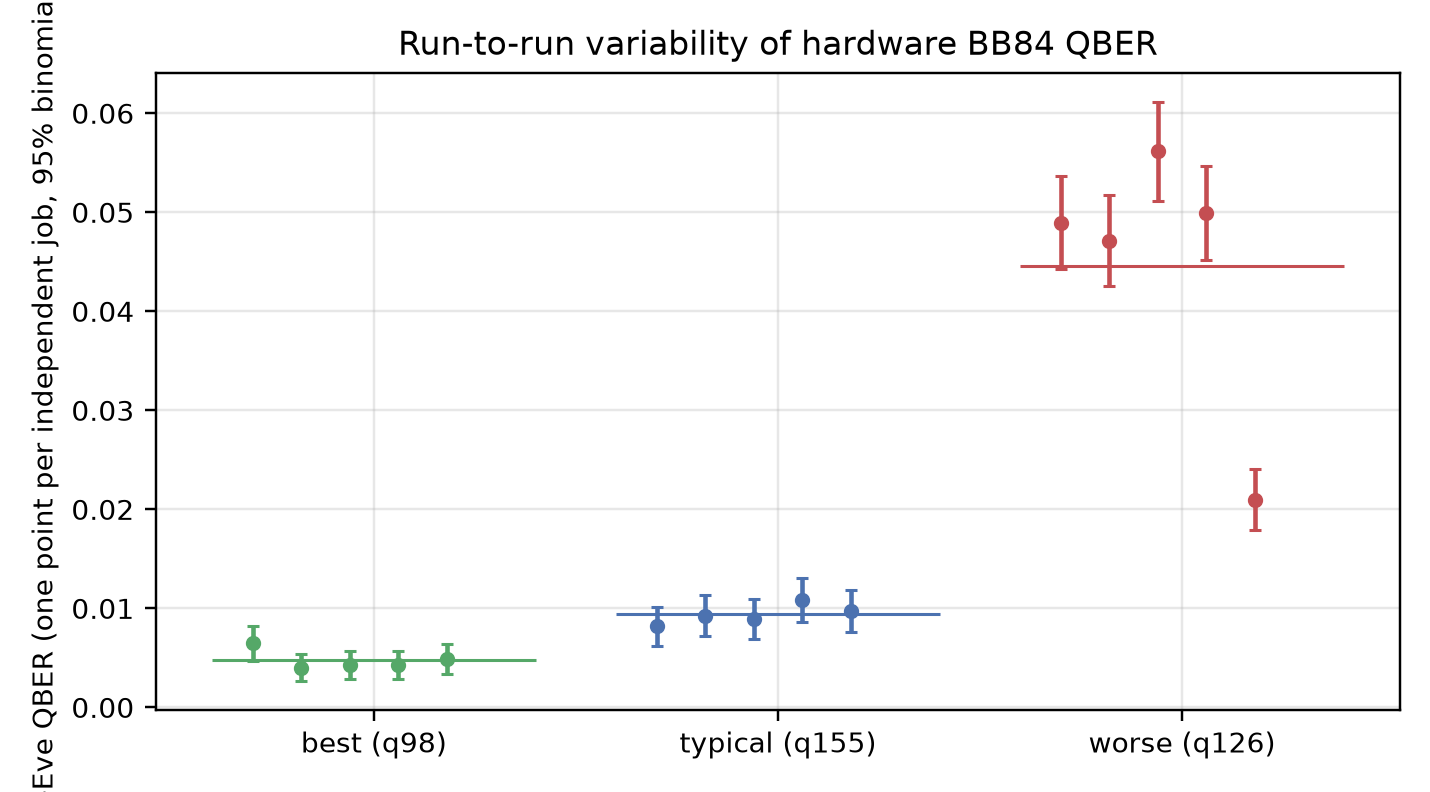
\includegraphics[width=\figw]{hw_qber_per_job}
\caption{Run-to-run variability of hardware no-Eve QBER: one point per independent job.}
\label{fig:hwjobs}
\end{figure}
\begin{figure}[t]
\centering
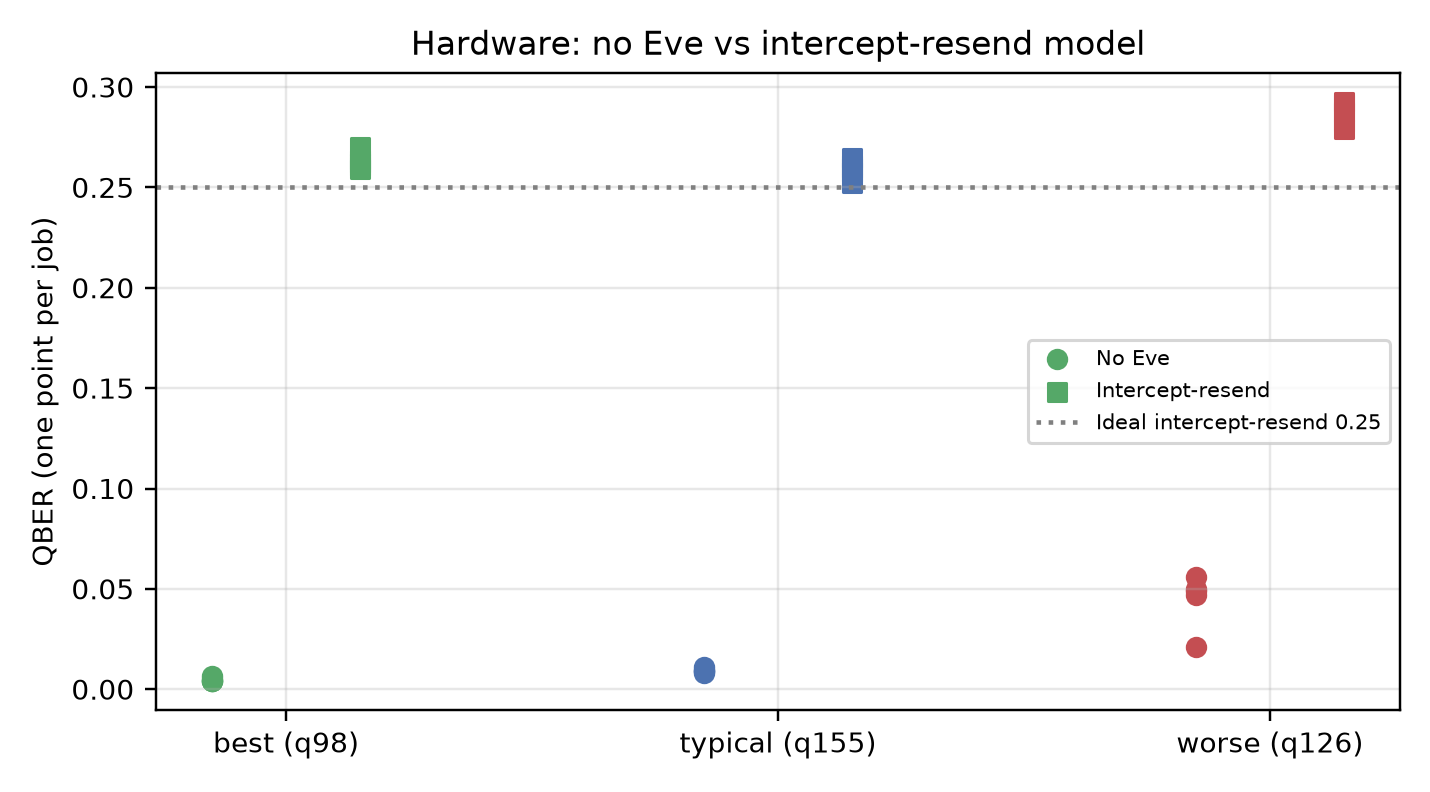
\includegraphics[width=\figw]{hw_eve_vs_noeve}
\caption{Hardware no-Eve versus intercept--resend-model QBER by job and qubit tier.}
\label{fig:hweve}
\end{figure}

\subsection{State asymmetry and simulator prediction}
The pilot suggested larger error for $|1\rangle$-prepared states. In the replicated data, $P(\text{misread}\mid |1\rangle)$ exceeded $P(\text{misread}\mid |0\rangle)$ in \HwAsymCells{} job-by-qubit cells: on the best qubit the values were \HwAsymZeroBest{} for $|0\rangle$ and \HwAsymOneBest{} for $|1\rangle$, but on the worse qubit the pattern reversed (\HwAsymZeroWorse{} versus \HwAsymOneWorse{}). The asymmetry is therefore qubit-dependent; it is consistent with relaxation and asymmetric readout effects, but no unique cause is established. Backend-derived noisy Aer predicted hardware QBER with MAE \HwNoisyMAE{} and RMSE \HwNoisyRMSE{} over 36 circuit-by-qubit cells (ideal Aer: MAE \HwIdealMAE{}); it over-predicted error on the worse qubit, and it used backend properties at analysis time rather than at job time.

\begin{figure}[t]
\centering
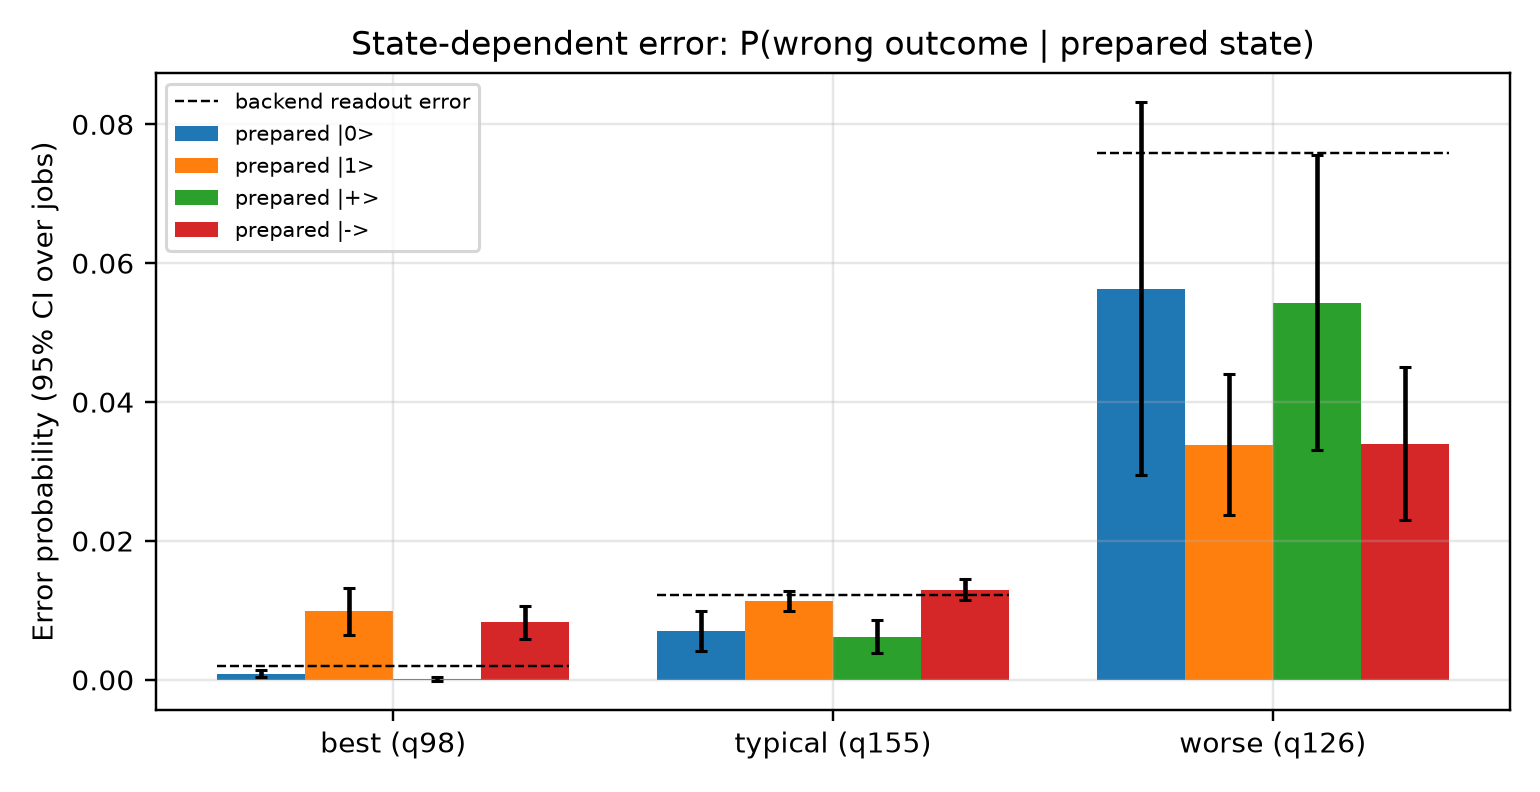
\includegraphics[width=\figw]{hw_state_asymmetry}
\caption{State-dependent misreads by qubit tier, with backend readout error (dashed).}
\label{fig:hwasym}
\end{figure}
\begin{figure}[t]
\centering
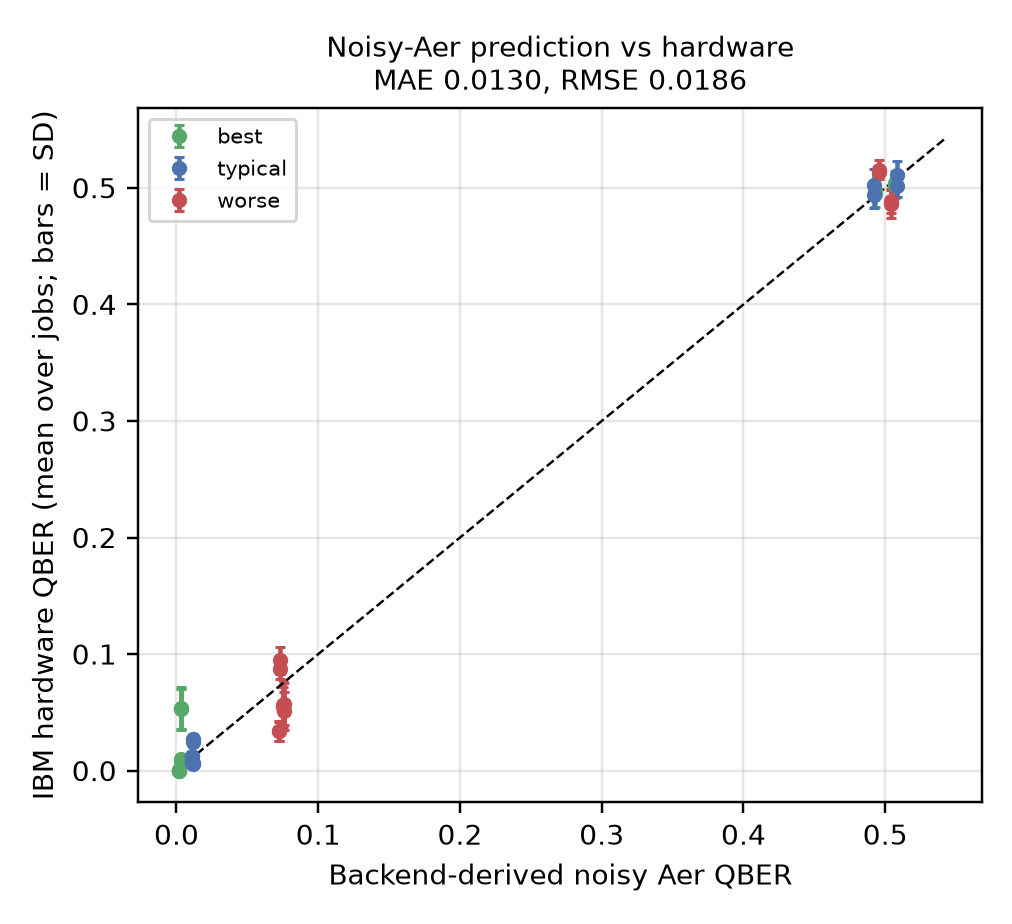
\includegraphics[width=\figw]{hw_noisy_aer_vs_hardware}
\caption{Noisy-Aer prediction versus hardware QBER per circuit and qubit tier.}
\label{fig:hwnoisy}
\end{figure}

\subsection{Grover and transpilation}
A two-qubit Grover search over four items with marked state $|11\rangle$ (ideal success 1) reached a pooled hardware success probability of \HwGroverPooled{}. By optimization level 0 to 3 the hardware success was \HwGroverOptZero{}, \HwGroverOptOne{}, \HwGroverOptTwo{} and \HwGroverOptThree{} (noisy Aer about \HwGroverNoisyOne{}), with transpiled depths \HwGroverDepthZero{}, \HwGroverDepthOne{}, \HwGroverDepthTwo{}, \HwGroverDepthThree{} and \HwGroverTwoQOne{} two-qubit gates at every level; differences between levels are small relative to between-job variation, so no optimization-level trend is claimed. This is an educational demonstration with no implication for AES or RSA key sizes; Shor's algorithm was not implemented.

\begin{table}[t]
\centering
\small
\caption{Two-qubit Grover (marked state $|11\rangle$): success probability by transpiler optimization level (5 independent jobs).}
\label{tab:hw-grover}
\resizebox{\linewidth}{!}{%
\begin{tabular}{rrrrrrrr}
\toprule
Opt. level & Depth & 2Q gates & HW success & CI low & CI high & Noisy Aer & Ideal Aer \\
\midrule
0 & 14 & 2 & 0.9465 & 0.9357 & 0.9573 & 0.9673 & 1.0000 \\
1 & 12 & 2 & 0.9521 & 0.9454 & 0.9589 & 0.9680 & 1.0000 \\
2 & 10 & 2 & 0.9441 & 0.9303 & 0.9580 & 0.9680 & 1.0000 \\
3 & 10 & 2 & 0.9412 & 0.9318 & 0.9506 & 0.9680 & 1.0000 \\
\bottomrule
\end{tabular}}
\end{table}

\begin{figure}[t]
\centering
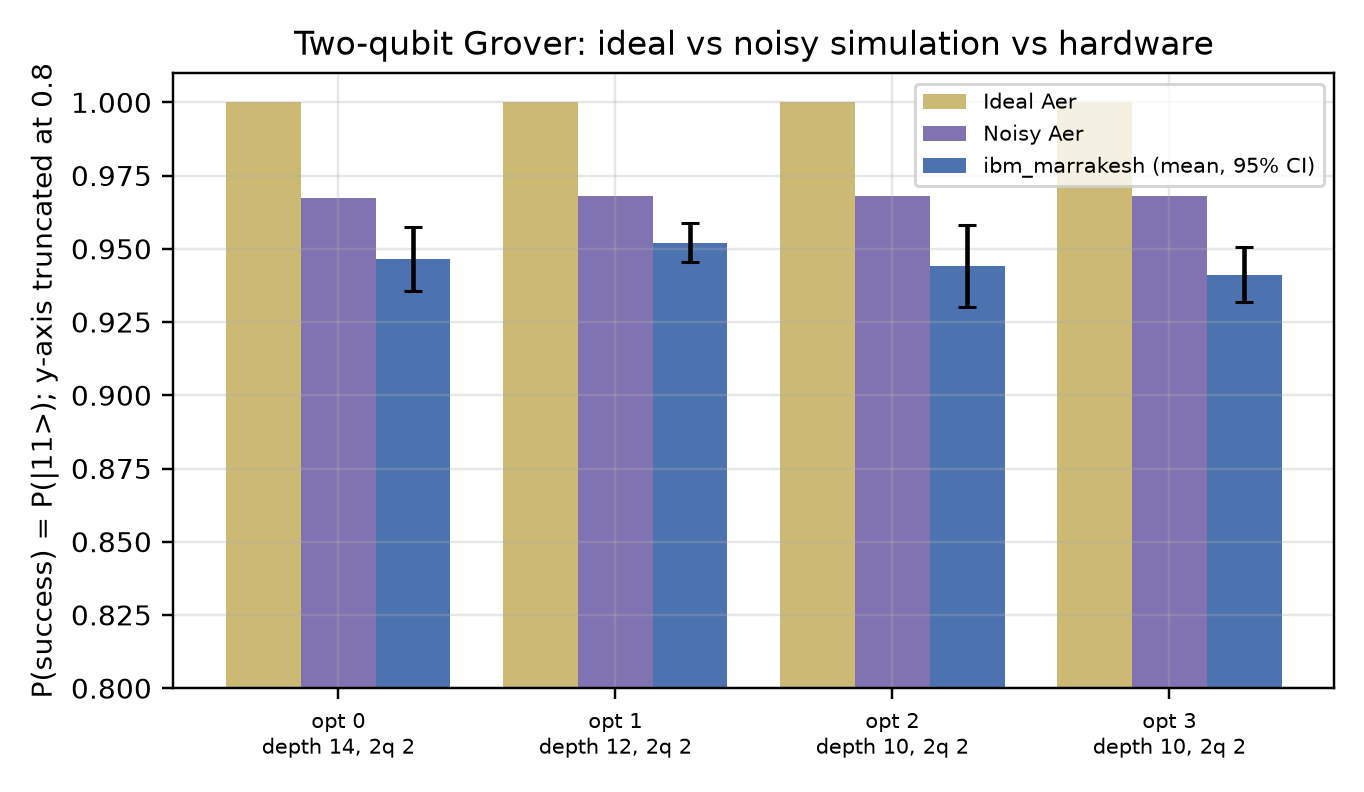
\includegraphics[width=\figw]{hw_grover_success}
\caption{Two-qubit Grover success probability: ideal Aer, noisy Aer and hardware.}
\label{fig:hwgrover}
\end{figure}

\subsection{QML circuits on \texttt{ibm\_fez}}
The CLT-QNN and linear-QNN circuits (4 qubits) with simulator-trained, frozen weights were bound to six held-out transactions and executed once. Mean absolute deviation between hardware and simulator expectation values was \FezCltMAD{} (Chow--Liu, transpiled depth \FezCltDepth{}) and \FezLinearMAD{} (linear, depth \FezLinearDepth{}), with hardware outputs strongly compressed toward zero for the deeper linear circuit. This supports only the limited claim that the circuits are physically executable and that hardware outputs differ markedly from simulation (more so for the deeper circuit; two circuits only); it is not evidence of a hardware predictive advantage, and the training experiment itself is simulator-based.

\chapter{Discussion}
\section{Discussion}\label{sec:disc}
\paragraph{Quantum model design versus system value.} The observable-locality result is a statistically supported, architecture-level finding under the evaluated conditions; it did not translate into incremental value once a matched classical nonlinear control and XGBoost were present. Reporting both outcomes is the point of the design: improved quantum model design is not the same as quantum predictive advantage.

\paragraph{Implementation versus primitive cost.} Compiling the post-quantum primitives removed most of the measured latency for ML-KEM and for ML-DSA key generation and verification, but not for ML-DSA signing or SLH-DSA-128s signing. Operational feasibility conclusions about post-quantum migration should therefore be stated per primitive and per implementation. The \texttt{pqcrypto} build is compiled but not necessarily the most heavily optimized code path available, so its numbers are an upper bound on what a tuned native library might achieve and are not a claim about \texttt{liboqs}.

\paragraph{BB84 evidence.} Two independent software implementations agree to within a maximum mean-QBER difference of \BbMaxDiff{} and reproduce the expected clean, noisy and intercept--resend behaviour. The IBM runs add a different kind of evidence: calibration-dependent hardware error is of the same order as moderate channel noise, but the intercept--resend model remains distinguishable from it. Neither is physical QKD.

\paragraph{Threshold choice.} A fixed QBER threshold trades missed detections against false alarms when noise varies; the value must be set for the expected channel noise rather than treated as a universal constant.

\chapter{Limitations}
\section{Limitations and Threats to Validity}\label{sec:limits}
\begin{itemize}
\item \textbf{No physical QKD, photons or quantum network.} BB84 is software-simulated at protocol and circuit level; IBM runs are circuit-level hardware validation.
\item \textbf{Hardware scope.} Selected circuits on one backend (\HwBackend{}), five jobs within a single session and calibration window; temporal replication across calibration periods was not performed. Results depend on backend, calibration, qubit mapping, transpilation and execution time. Only three qubits were compared, so no correlation with calibration quality is claimed. The noisy-Aer model used properties at analysis time.
\item \textbf{Full QSFD not on hardware.} The fraud classifier was trained and evaluated in simulation; the earlier \path{ibm_fez} run executed six inference circuits only.
\item \textbf{PQC backends.} Native \texttt{liboqs} could not be built (no CMake/MSVC); \texttt{pqcrypto} is a compiled but not necessarily AVX2-optimized build; absolute latencies are machine-specific, and repetition counts differ between backends (reference SLH-DSA signing $n=3$). The earlier ${\sim}15$~s reference figure was measured in another session and is not reproduced here.
\item \textbf{End-to-end experiment.} In-memory transmission only; long-term keys assumed pre-distributed; no concurrency, load or HSM integration.
\item \textbf{BB84 simulations.} Different noise models in the two simulators; Qiskit trials used 500 bits (not 2000) for runtime; the detection-threshold optimum depends on the noise range chosen.
\item \textbf{Data.} A single public dataset with 0.17\% fraud prevalence; quantum experiments use a rebalanced controlled subset; no real bank data or production deployment.
\item \textbf{Layer~3.} Shor's algorithm is not implemented; the two-qubit Grover circuit says nothing about attacks on AES or RSA key sizes.
\item \textbf{Internal/external/construct validity.} Seeds, splits, benchmark noise and hardware variability are controlled but not eliminated; conclusions are limited to the evaluated configurations, and the reference-versus-compiled comparison measures implementations, not security levels.
\end{itemize}

\chapter{Conclusion and Future Work}
\section{Conclusion and Future Work}\label{sec:concl}
Under the evaluated conditions, (i) a local-sum observable significantly improves a matched quantum neural network, but no incremental quantum predictive value over XGBoost or a classical control was verified; (ii) a compiled backend lowers PQC latency by \SpeedupMin{}--\SpeedupMax{}$\times$ depending on the operation, with SLH-DSA-128s signing remaining costly; (iii) two independent BB84 simulations agree closely and reproduce the expected eavesdropping signature; and (iv) selected circuits executed on IBM Quantum hardware show measurable, calibration-dependent error relative to ideal and noisy simulation while keeping the intercept--resend model distinguishable. No quantum advantage, physical QKD, or practical attack on RSA or AES is claimed. Future work: a native \texttt{liboqs} comparison on a toolchain-equipped machine, replication across backend calibration periods and devices, a Shor implementation, adversarial-ML attacks in Layer~3, and evaluation on real transaction streams.

\chapter{Environment, Reproduction and Test Summary}
\section*{Environment and versions}
Operating system Windows~11; Python~3.14; Qiskit~2.5.2; Qiskit Aer~0.17.2; \texttt{pqcrypto}~\PqcryptoVersion{}; full metadata in \path{results/final/final_results.json} and \path{results/layer2/pqc_benchmark_meta.json}. Native \texttt{liboqs}: not operational (no CMake/MSVC); no liboqs measurements.

\section*{Test summary}
Total \TestsTotal{}; passed \TestsPassed{}; failed \TestsFailed{}; skipped \TestsSkipped{}.

\section*{Reproduction commands}
\begin{itemize}[noitemsep]
\item \path{python scripts/security/run_pqc_backend_benchmarks.py}
\item \path{python scripts/security/run_end_to_end_banking.py}
\item \path{python scripts/security/run_bb84_final.py}
\item \path{python scripts/ibm_quantum/analyze_campaign.py A} (saved artifacts only; no hardware quota)
\item \path{python scripts/final/build_final_results.py} then \path{python scripts/final/build_latex_assets.py}
\end{itemize}

\section*{IBM job provenance}
Pilot: \path{ibm_marrakesh} job \HwPilotJob{}. Campaign A: five jobs listed in \path{results/final/final_results.json} (field \path{ibm_quantum.campaign.job_ids}). QML run: \path{ibm_fez} job \HwFezJob{}.

\section*{Algorithm name mapping}
ML-KEM (FIPS~203, from CRYSTALS-Kyber), ML-DSA (FIPS~204, from CRYSTALS-Dilithium), SLH-DSA (FIPS~205, from SPHINCS+). Reference identifiers: \path{ML_KEM_768}, \path{ML_DSA_65}, \path{sha2_128s}; \texttt{pqcrypto} modules: \path{pqcrypto.kem.ml_kem_768}, \path{pqcrypto.sign.ml_dsa_65}, \path{pqcrypto.sign.slh_dsa_sha2_128s}.


% ---- bibliography: no header ----
\clearpage
\pagestyle{nohdr}
\fancypagestyle{plain}{\fancyhf{}\renewcommand{\headrulewidth}{0pt}\fancyfoot[L]{\hf\projtitle}\fancyfoot[R]{\hf\thepage}}
\renewcommand{\bibname}{BIBLIOGRAPHY}
\addcontentsline{toc}{chapter}{Bibliography}
\chapter*{Bibliography}
\begin{thebibliography}{99}
\setstretch{1.5}
\bibitem{shor} Peter W. Shor, \textquotedblleft{}Polynomial-Time Algorithms for Prime Factorization and Discrete Logarithms on a Quantum Computer\textquotedblright{}, \textit{SIAM Journal on Computing}, vol. 26, no. 5, 1997, pp. 1484--1509, \textit{doi:10.1137/S0097539795293172}.
\bibitem{mosca} Michele Mosca, \textquotedblleft{}Cybersecurity in an Era with Quantum Computers: Will We Be Ready?\textquotedblright{}, \textit{IEEE Security \& Privacy}, vol. 16, no. 5, 2018, pp. 38--41, \textit{doi:10.1109/MSP.2018.3761723}.
\bibitem{nist203} National Institute of Standards and Technology, \textquotedblleft{}FIPS 203: Module-Lattice-Based Key-Encapsulation Mechanism Standard\textquotedblright{}, \textit{NIST}, 2024, \textit{doi:10.6028/NIST.FIPS.203}.
\bibitem{nist204} National Institute of Standards and Technology, \textquotedblleft{}FIPS 204: Module-Lattice-Based Digital Signature Standard\textquotedblright{}, \textit{NIST}, 2024, \textit{doi:10.6028/NIST.FIPS.204}.
\bibitem{nist205} National Institute of Standards and Technology, \textquotedblleft{}FIPS 205: Stateless Hash-Based Digital Signature Standard\textquotedblright{}, \textit{NIST}, 2024, \textit{doi:10.6028/NIST.FIPS.205}.
\bibitem{xgboost} Tianqi Chen and Carlos Guestrin, \textquotedblleft{}XGBoost: A Scalable Tree Boosting System\textquotedblright{}, \textit{Proc. 22nd ACM SIGKDD Int. Conf. Knowledge Discovery and Data Mining}, 2016, pp. 785--794, \textit{doi:10.1145/2939672.2939785}.
\bibitem{havlicek} None, \textquotedblleft{}Supervised Learning with Quantum-Enhanced Feature Spaces\textquotedblright{}, \textit{Nature}, vol. 567, 2019, pp. 209--212, \textit{doi:10.1038/s41586-019-0980-2}.
\bibitem{schuld} Maria Schuld and Nathan Killoran, \textquotedblleft{}Quantum Machine Learning in Feature Hilbert Spaces\textquotedblright{}, \textit{Physical Review Letters}, vol. 122, no. 4, 2019, pp. 040504, \textit{doi:10.1103/PhysRevLett.122.040504}.
\bibitem{bb84} Charles H. Bennett and Gilles Brassard, \textquotedblleft{}Quantum Cryptography: Public Key Distribution and Coin Tossing\textquotedblright{}, \textit{Proc. IEEE Int. Conf. Computers, Systems and Signal Processing}, 1984, pp. 175--179.
\bibitem{liboqs} Open Quantum Safe project, \textquotedblleft{}Open Quantum Safe project: liboqs and liboqs-python\textquotedblright{}, \textit{https://openquantumsafe.org}.
\bibitem{pqcrypto} pqcrypto contributors, \textquotedblleft{}pqcrypto: Python bindings for post-quantum cryptography\textquotedblright{}, \textit{Python Package Index, version 1.0.0, 2026}.
\bibitem{bolton} Richard J. Bolton and David J. Hand, \textquotedblleft{}Statistical Fraud Detection: A Review\textquotedblright{}, \textit{Statistical Science}, vol. 17, no. 3, 2002, pp. 235--255, \textit{doi:10.1214/ss/1042727940}.
\bibitem{ngai} E. W. T. Ngai, Yong Hu, Y. H. Wong, Yijun Chen, and Xin Sun, \textquotedblleft{}The Application of Data Mining Techniques in Financial Fraud Detection: A Classification Framework and an Academic Review of Literature\textquotedblright{}, \textit{Decision Support Systems}, vol. 50, no. 3, 2011, pp. 559--569, \textit{doi:10.1016/j.dss.2010.08.006}.
\bibitem{haixiang} Guo Haixiang, Li Yijing, Jennifer Shang, Gu Mingyun, Huang Yuanyue, and Gong Bing, \textquotedblleft{}Learning from Class-Imbalanced Data: Review of Methods and Applications\textquotedblright{}, \textit{Expert Systems with Applications}, vol. 73, 2017, pp. 220--239, \textit{doi:10.1016/j.eswa.2016.12.035}.
\bibitem{dalpozzolo} Andrea Dal Pozzolo, Olivier Caelen, Reid A. Johnson, and Gianluca Bontempi, \textquotedblleft{}Calibrating Probability with Undersampling for Unbalanced Classification\textquotedblright{}, \textit{Proc. IEEE Symposium Series on Computational Intelligence (SSCI)}, 2015, pp. 159--166, \textit{doi:10.1109/SSCI.2015.33}.
\bibitem{cerezo} M. Cerezo, Akira Sone, Tyler Volkoff, Lukasz Cincio, and Patrick J. Coles, \textquotedblleft{}Cost Function Dependent Barren Plateaus in Shallow Parametrized Quantum Circuits\textquotedblright{}, \textit{Nature Communications}, vol. 12, 2021, pp. 1791, \textit{doi:10.1038/s41467-021-21728-w}.
\bibitem{kyriienko} Oleksandr Kyriienko and Einar B. Magnusson, \textquotedblleft{}Unsupervised Quantum Machine Learning for Fraud Detection\textquotedblright{}, \textit{arXiv:2208.01203}, 2022.
\bibitem{chowliu} C. K. Chow and C. N. Liu, \textquotedblleft{}Approximating Discrete Probability Distributions with Dependence Trees\textquotedblright{}, \textit{IEEE Transactions on Information Theory}, vol. 14, no. 3, 1968, pp. 462--467, \textit{doi:10.1109/TIT.1968.1054142}.
\bibitem{grover} Lov K. Grover, \textquotedblleft{}A Fast Quantum Mechanical Algorithm for Database Search\textquotedblright{}, \textit{Proc. 28th Annual ACM Symposium on Theory of Computing (STOC)}, 1996, pp. 212--219, \textit{doi:10.1145/237814.237866}.
\bibitem{nistir8105} Lily Chen, Stephen Jordan, Yi-Kai Liu, Dustin Moody, Rene Peralta, Ray Perlner, and Daniel Smith-Tone, \textquotedblleft{}Report on Post-Quantum Cryptography\textquotedblright{}, \textit{NIST, NISTIR 8105}, 2016, \textit{doi:10.6028/NIST.IR.8105}.
\bibitem{kyber} Joppe Bos, Leo Ducas, Eike Kiltz, Tancrede Lepoint, Vadim Lyubashevsky, John M. Schanck, Peter Schwabe, Gregor Seiler, and Damien Stehle, \textquotedblleft{}CRYSTALS-Kyber: A CCA-Secure Module-Lattice-Based KEM\textquotedblright{}, \textit{Proc. IEEE European Symposium on Security and Privacy (EuroS\&P)}, 2018, pp. 353--367, \textit{doi:10.1109/EuroSP.2018.00032}.
\bibitem{dilithium} Leo Ducas, Eike Kiltz, Tancrede Lepoint, Vadim Lyubashevsky, Peter Schwabe, Gregor Seiler, and Damien Stehle, \textquotedblleft{}CRYSTALS-Dilithium: A Lattice-Based Digital Signature Scheme\textquotedblright{}, \textit{IACR Transactions on Cryptographic Hardware and Embedded Systems}, vol. 2018, no. 1, 2018, pp. 238--268, \textit{doi:10.46586/tches.v2018.i1.238-268}.
\bibitem{sphincs} Daniel J. Bernstein, Andreas Hulsing, Stefan Kölbl, Ruben Niederhagen, Joost Rijneveld, and Peter Schwabe, \textquotedblleft{}The SPHINCS+ Signature Framework\textquotedblright{}, \textit{Proc. ACM SIGSAC Conf. Computer and Communications Security (CCS)}, 2019, pp. 2129--2146, \textit{doi:10.1145/3319535.3363229}.
\bibitem{shorpreskill} Peter W. Shor and John Preskill, \textquotedblleft{}Simple Proof of Security of the BB84 Quantum Key Distribution Protocol\textquotedblright{}, \textit{Physical Review Letters}, vol. 85, no. 2, 2000, pp. 441--444, \textit{doi:10.1103/PhysRevLett.85.441}.
\bibitem{gisin} Nicolas Gisin, Gregoire Ribordy, Wolfgang Tittel, and Hugo Zbinden, \textquotedblleft{}Quantum Cryptography\textquotedblright{}, \textit{Reviews of Modern Physics}, vol. 74, no. 1, 2002, pp. 145--195, \textit{doi:10.1103/RevModPhys.74.145}.
\bibitem{preskill} John Preskill, \textquotedblleft{}Quantum Computing in the NISQ Era and Beyond\textquotedblright{}, \textit{Quantum}, vol. 2, 2018, pp. 79, \textit{doi:10.22331/q-2018-08-06-79}.
\bibitem{qiskit} Ali Javadi-Abhari and others, \textquotedblleft{}Quantum Computing with Qiskit\textquotedblright{}, \textit{arXiv:2405.08810}, 2024.
\bibitem{efron} B. Efron, \textquotedblleft{}Bootstrap Methods: Another Look at the Jackknife\textquotedblright{}, \textit{The Annals of Statistics}, vol. 7, no. 1, 1979, pp. 1--26, \textit{doi:10.1214/aos/1176344552}.
\bibitem{wilcoxon} Frank Wilcoxon, \textquotedblleft{}Individual Comparisons by Ranking Methods\textquotedblright{}, \textit{Biometrics Bulletin}, vol. 1, no. 6, 1945, pp. 80--83, \textit{doi:10.2307/3001968}.
\bibitem{nielsen} Michael A. Nielsen and Isaac L. Chuang, \textquotedblleft{}Quantum Computation and Quantum Information\textquotedblright{}, Cambridge University Press, 10th Anniversary ed., 2010.
\end{thebibliography}

\end{document}
